\documentclass[master]{IPSstyle}

  \Year{2017}
  \Month{February}
  \Author{44151020-2: ZHAO, Xuan}
  \Title{Random Forest Based Quasi-Linear Kernel Composition for \\Support Vector Machine}

  \Advisor{Professor Jinglu Hu}

\usepackage{amssymb,amsmath}

\usepackage{mathptmx}
\usepackage{helvet}
\usepackage{courier}
\usepackage{type1cm}

\usepackage{makeidx}
\usepackage{graphicx,subfigure}
\usepackage{multicol}
\usepackage{multirow}
\usepackage[bottom]{footmisc}

\usepackage{mathrsfs}
\usepackage{amssymb,amsmath}
\usepackage{amsfonts}
\usepackage{color}
\usepackage{CJKutf8}
\usepackage{flowchart}
\usepackage{float}
\usepackage{tikz}
\usetikzlibrary{shapes.geometric, arrows}

\newtheorem{remark}{Remark}
\usepackage{listings}
\usepackage{algorithm,algorithmicx,algpseudocode}
\usepackage[toc,page,title,titletoc,header]{appendix}

\renewcommand{\algorithmicrequire}{\textbf{Input:}}
\renewcommand{\algorithmicensure}{\textbf{Output:}}

\newtheorem{theorem}{Theorem}
\newtheorem{lemma}[theorem]{Lemma}
\newtheorem{proposition}[theorem]{Proposition}
\newtheorem{corollary}[theorem]{Corollary}
\newtheorem{definition}{Definition}



\Abstract{
Object recognition and classification are one of the most fundamental and representative problems in the artificial intelligence filed. The overcome of such problem will be significant and meaningful. By tons of researches and experiences, it is commonly believed that two factors are essential for the performance of object recognition and classification. They are abstract feature representation and algorithm to optimize a given problem. On the one hand, feature representation, as the only way for a computer to know the real world, determines the upper bound of the potential intelligent level. On the other hand, for a given feature representation and a specific situation, the effectiveness of an algorithm decides the approaching level of the potential upper bound. Therefore, feature representation and algorithm formulation are always two hot topics in the artificial intelligence filed.

In this paper, starting from analysis and summarize the algorithm formulation for classification tasks, local linearity detection is implemented to improve a previously proposed model. Based on it, a local linearity detection based quasi-linear support vector machine is proposed. A quasi-linear here means the nonlinear separation boundary is approximated by using multi-local linear boundaries with interpolation. This thesis proposes a flexible way to construct a quasi-linear kernel by combining the matured ensemble learning method, analysis, and simulation experiments are conducted for exploration of the suitable applications of the proposed method. 

Firstly, based on a certain criterion, we train lots of decision trees with resampling data set and random feature subsets. Secondly, we get lots of set of local linear information. Then, after doing cluster, the final information is embedded into the composition of a quasi-linear kernel with the original data set. At last, a global optimization is implemented to train a final classifier.

Experimental results on synthetic datasets show that our proposed method is flexible to capture the potential classification boundary for specific problems, while the experiments in real-world data sets demonstrate improvements of classification performances over traditional classifiers.
}

\Keywords{support vector machine, quasi-linear kernel function, random forest}

\Acknowledgments{
   It is quite an unforgettable time I spend in here, Furuzuki Lab, Waseda University. I, at here, sincerely express my gratitude to my professor, Jinglu Hu, who devoting himself to supervising us. Professor HU is not only knowledgeable but also very willing to help us in daily life. It is a great honor for me to be a member of his Lab.
   
   I would also like to thank Bo Zhou, Weite Li and many other students in Furuzuki Lab who have provided their valuable opinions and assistance to me in my whole master period.

   At last, thanks to all my friends and my parents for their great support and companion, this paper can not be finished without their patient to comfort me.
}

\begin{document}

 \makepreliminarypages
 \singlespace
 \frontmatter
 \tableofcontents
 \listoffigures
 \listoftables
 \mainmatter
 \clearemptydoublepage
 \setlength{\baselineskip}{23.0pt}

\chapter{Introduction}

In this thesis, a flexible way based on ensemble learning method to compose a quasi-linear kernel for support vector machine is proposed for a better performance of binary classification tasks. In this chapter, firstly, we will introduce the background of machine learning field and it's significant. Next, we will introduce the related works of this thesis. Then, the motivations and the purpose of this method will be presented. Last, the structure of this thesis will be laid out to give a perspective view.  

\section{Machine Learning for Classification}
As a way of realizing artificial intelligence, machine learning has been widely accepted and practiced with the help of the modern computer. As an important subject in the field of machine learning, the problem of classification has been paid high attention to the experts in the field since the birth of machine learning.

Classification problem is defined as that building a model under given data distribution, then making the computer can automatically classify input data and give it a class tag~\cite{bishop2006pattern}.  For example, the image stored in computer memory just a bunch of binary numbers which humans can not understand. However, the computer could extract some clear features of the characteristics from the given original binary numbers by learning algorithm, and the relevance of these features is the key components to rebuild a specific image. So, once we have the feature extraction method and tagged label information for each image, and then split these image data set into the training set and test set. Then, the computer can use the training set for classifier learning, using the test set to test the performance of the trained classifier. Therefore, if we can design an effective learning algorithm, the computer will be able to self-learning, get the capability of automatic classification of different images~\cite{krizhevsky2012imagenet}.

Generally speaking, classification problems can be categorized into supervised learning and unsupervised learning. In a supervised setting, a corresponding learning process is conducted with the help of not only input patterns but also their labels. However, in an unsupervised setting, only input patterns are provided for the learning process. By a simple comparison, the learning processes of supervised learning contain much more information of samples, so attract major attentions from researchers. In this thesis, supervised learning is our major concern.

There are so many discriminative supervised learning technologies in the machine learning field, such as logistic regression~\cite{menard2002applied}, support vector machines~\cite{cortes1995support,vapnik2000nature}, neural networks~\cite{hornik1989multilayer} and so on.  Unlike other methods, SVM uses structural risk minimization criteria to minimize the upper bound of the generalization error rather than simply reducing the model's training error. Moreover, the optimization process of an SVM is a convex optimization process, so it can guarantee a global minimum solution. Besides, SVM introduces a kernel trick~\cite{scholkopf2001learning}, which could map the original feature space to a very high dimension feature space. By ensuring the linear separability of the input samples in the high dimensional space, the SVM is promoted from a powerful linear classifier to a more powerful nonlinear classifier. For these reasons, SVM has received extensive attention in industry and academia for its excellent performance in classification. 

However, it is worth noting that since the traditional kernel functions (such as radial basis function) construct only a black box mapping for spatial variation, it does not take into account the structural information of the input data itself. Therefore, in the traditional mapping of kernel functions, the actual samples, and the noise samples will be simultaneously mapped to linearly separable high-dimensional space. As a result, the traditional SVM will inevitably have the problem of over-fitting, that is, the final classification boundary will over-fit the noise distribution and can not match the potential structure of the actual samples distribution itself. In the situation of high noise data or the number of samples is close to or much larger than the number of samples, the over-fitting problem is particularly severe.~\cite{barutcuoglu2006hierarchical,diplaris2005protein}. 

Inspired by the use of piecewise linear classifier approximating nonlinear boundary hyperplane, SVM based on quasi-linear kernel function is used to solve the over-fitting problem~\cite{chen2012composite, bo2014quasi}. By using the local linear information extracted from the feature space of the samples in the kernel function, the constructed kernel function can express the mapping method of the original input sample, and can also describe the actual physical meaning in the mapping process. 

After searching a lot of literature and exploring related methods, it is concluded that the robustness of local linear information directly determines the final training effect of quasi-linear kernel support vector machine. In view of this, this thesis proposes an ensemble learning method based on decision forest. The local linear information of the input samples learned by this method is taken as the core component of the composition of the quasi-linear kernel function. 

\section{Related Methods}
In order to solve the problem of over-fitting of kernel-based SVM in training process, the idea of constructing a combinational linear hyperplane to approximate non-linear hyperplane by using multiple SVMs is explored. But this type of SVM still could not guarantee the solution is globally optimal.

In the literature~\cite{hu2001quasi}, J. Hu et al. (2001) proposed a quasi-linear ARX model to identify a non-linear system. The quasi-linear ARX model can be regarded as a nonlinear approximation model with multiple interpolated linear models and has good generalization ability in the identification of nonlinear systems~\cite{chen2010local}. The model was latter extended to a quasi-linear support vector machine for solving classification problem~\cite{chen2010local, hu2001quasi}. By this way, they transform the PLC models from multiple local linear models optimization process to kernel function optimization so that the final non-linear classifier is just one SVM. Because we are aiming at a support vector machine optimization process, we can guarantee that the solution is a globally optimal solution. 

Therefore, in this thesis, we focus on this kernel way to construct a multi-local linear classifier, namely quasi-linear kernel SVM. Firstly, let's talk about the relative branch of SVMs research briefly, namely, using piecewise linear classifier approximating nonlinear boundary hyperplane.

\subsection{Unsupervised learning method}
Unsupervised learning method which doesn’t use label information, such as Kmeans, KNN, Manifold Learning methods.
H. Zhang proposed a method which using K-nearest neighbor algorithm, for each sample in the test set, find the adjacent K samples in the train set to construct a local linear classifier~\cite{zhang2006svm} . By this method, the SVM is transformed from global optimization to local optimization to reduce the complexity of the model and improve the performance of the classifier by using local linear separable properties. H. Cheng proposed a method which is to construct multiple linear classifiers in the training data set and each linear classifier corresponds to a subspace in the test samples feature space and ensure that the positive and negative samples in these subspaces can be separable by a linear hyperplane~\cite{cheng2010efficient}.
Since multiple linear SVM have the advantages that they are locally robust, for some noisy nonlinear classification problems, this type of methods may perform better than general nonlinear kernel SVMs~\cite{li2014growing}.

\subsection{Semi-supervised learning method}
In semi-supervised learning method, B.Zhou proposed a modified k-means method which also considers the information of label and proportion of label~\cite{bo2014quasi}. Firstly, by introducing the label information of the samples into the K-means algorithm, the division of the sample feature space is obtained, and then all the training samples are clustered. The local linear partitions information are used to construct the quasi-linear kernel function, and the global optimization can be ensured as well as the traditional support vector machine (SVM). 

\subsection{Supervised learning method}
In this kind of work, a supervised method would be more suitable for the determination of local partitions (we will discuss it in the next chapter). Therefore, it is highly motivated to develop a more sophisticated method to detect them properly. In the previous work, the geometric method could achieve better results~\cite{li2015geometric}.

\section{Motivation}
So far, we already know the kernel way to construct a multiple local linear classifier could have better performance than other ways in theoretic reason. However, two important issues that need to be addressed for local linear classifiers.
\begin{remark}\label{mark:dectect_linear}
\noindent How to detect the potential local linearity information.
\end{remark}
\begin{remark}\label{mark:numM}
\noindent  It is still difficult to determine the number of local linear classifiers and their respective scopes.
\end{remark}

The major reason behind it is that a data-independent kernel function is hard to represent the complicated manifold where samples concentrate~\cite{bengio2013representation}. By this way, since we must construct a quasi-linear kernel function, we must first find a way to detect the local linearity and then, we also must know the number of local linear classifiers and their respective scopes. For this reason, \emph{the proposed method in this paper would give a more flexible and robust supervised algorithm for composition a quasi-linear kernel}.

It is expected that the information of local linearity can be firstly detected by our proposed method, which means that the number of local linear classifiers and their function scopes should be firstly determined by our method. After this, the information can be embedded into the composition of the quasi-linear kernel. Then, a global optimization can be expected to output a compelling result.

\section{Thesis Organization}
The remainder of this article is organized as follows: In Chapter 2, introduce the concepts, definitions and provide mathematical solutions of quasi-linear kernel SVM, and discuss the inner mechanism of the quasi-linear SVM. In chapter 3, several classical algorithms of a decision tree theory are introduced. Then show decision tree can be used to get local linear information. Next, we introduce random forest, which is a powerful extension to the decision tree algorithm in statistical machine learning aims to get a preciser local linear information for kernel construction. In Chapter 4, the feasibility and effectiveness of the proposed method are demonstrated by simulating experiments. Finally, conclusions are discussed in Chapter 5.

\chapter{Quasi-linear Support Vector Machines} \label{ch2}

In this chapter, we will first introduce the necessary contents of SVM, then introduce the related technology of quasi-linear vector machine, analyzes its working principle, and discusses the optimization approach of the quasi-linear kernel function.

\section{Support Vector Machine}
SVM as a supervised learning method~\cite{vapnik2000nature}, which is widely used in classification and regression problems. Because at that time its performance even surpassed the complex neural network system, therefore has caused the great attention and the research interest in the academic circle. Because it uses the optimization learning method developed from the statistical learning theory, it learns a linear classification function by using structural risk minimization criterion in the high-dimensional sample space. Compared with the empirical risk of traditional neural networks, the structural risk minimization criterion directly optimizes the upper limit of the expected risk, which shows the learning and generalization performance better than the risk minimization criterion.

\subsection{Support Vector Machine Optimization}
We start from basic case, given number of $L$ training samples, each sample contains a $d$ dimensional input signal  $(x_i \in \mathbf{R}^d)$ and a class label $(y_i \in {-1, 1})$. First, the hyperplane of all $\mathbf{R}^d$ spaces is represented by a vector $\omega$ and a constant $b$ as the following equation:
\begin{equation}
\omega^Tx+b=0
\end{equation}
where $\omega$ is a vector orthogonal to the hyperplane and $b$ is the bias of the hyperplane. Assuming a hyperplane to divide the data set, then have the following equation:
\begin{equation}
f(x) = sign(\omega^T x + b)
\end{equation}
In the case of linear separability, the hyperplane is defined as having a margin of at least unit one from the data set, namely the hyperplane satisfies the following condition:
\begin{align}
&\omega^T x_i + b \geq + 1 ~~~~~ \text{when} ~ y_i =+1 \\
&\omega^T x_i + b \leq -1 ~~~~~ \text{when} ~ y_i =- 1
\end{align}
Or just write as:
\begin{equation}
y_i \left( \omega^T x_i + b \right) \geq 1 ~\text{for} ~\forall i \label{eq2.5}
\end{equation}

In fact, $(\omega, b)$ and $(\lambda\omega, \lambda b)$ where $\lambda \in \mathbf{R}^+$ represent the same hyperplane, since each hyperplane has a different functional distance for a given training data set. Therefore, in order to get the distance between the hyperplane and the data set, we must normalize the length of vector w, that is, rewrite above formula as: 
\begin{equation}
d((\omega, b), x_i) = \frac{(\omega^T x_i + b)}{||\omega||} \geq \frac{1}{||w||}
\end{equation}
\begin{figure}[H]
  \centering
  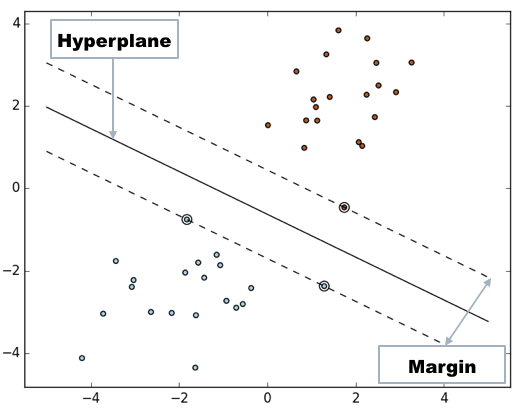
\includegraphics[width=11cm]{figures/ch2_support_vectors.png}
  \caption{Illustration of a hyperplane and maximum margin for a SVM} \label{fg:SVs}
\end{figure}
Thus, the optimal hyperplane can be defined as maximizing the margin between the hyperplane and the data set, as shown in the following figure \ref{fg:SVs}, circled points are called support vectors.

At this point, the support vector machine hyperplane optimization problem can be converted to maximum $\frac{1}{||w||}$under the constraints. In summary, the support vector machine optimization formulation can be written as follows:
\begin{equation}\label{eq:2:SVM_Primal}
\begin{aligned}
&\min_{\omega}  ~ \frac{1}{2}\Vert\omega\Vert^2\\
&s.t. ~ y_i\left(\omega^Tx_i+b\right)\geq1, ~ i=1,2,...,m
\end{aligned}
\end{equation}

This formula is a standard convex quadratic programming problem, although the results can be obtained directly by software, but if the input signal dimension is too large, will lead to the optimization process slowing down, and even lead to unenforceable. In order to solve such problem, the dual form of this formula is widely used.

According to Lagrangian duality, Lagrange Multiplier $\alpha_i, i = 1,2,\dots, m$ is introduced, formula~\ref{eq:2:SVM_Primal} could rewrite as:
\begin{equation}
L \left(\omega, \alpha, b\right) = \frac{1}{2}\Vert\omega\Vert^2 - \sum_{i=1}^m\alpha_i\left[y_i(\omega^Tx_i + b) - 1\right]
\end{equation}

In order to derive the dual form of the equation, first need to fix $\alpha_i$, then calculate the partial derivatives of $\omega, b$ to optimize $L(\omega, \alpha, \beta)$:
\begin{align}
\nabla_w L(\omega, b, \alpha) = \omega - \sum_{i=1}^m\alpha_iy_ix_i = 0 \\
\frac{\partial}{\partial b}L(\omega, b, \alpha) = \sum_{i=1}^m\alpha_iy_i = 0
\end{align}

According to Karush-Kuhn-Tucker conditions (KKT), we could know the primal and dual problem are the same solutions in SVM. So, we could get the dual optimization formulation of support vector machine finally:
\begin{equation} \label{eq:2:SVM_dual}
\begin{aligned}
\max_{\alpha} ~ &W(\alpha)=\sum_{i=1}^{m}\alpha_i-\frac{1}{2}\sum_{i,j=1}^{m}y_iy_j\alpha_i\alpha_j<x_i,x_j>\\
s.t. ~ &\alpha_i\geq0, ~ i=1,2,...,m\\
&\sum_{i=1}^{m}\alpha_iy_i=0
\end{aligned}
\end{equation}

After solving parameter of $\alpha_i$, then we can solve $\omega$ from formula~\ref{eq:2:SVM_dual}, finally get $b$ from the formula below:
\begin{equation}
b^\ast = -\frac{\max_{y_i=-1}\omega^{\ast T}x_i + \min_{y_i=1}\omega^{\ast T}x_i}{2}
\end{equation}

Finally, using formula 2.2 calculate $f(x)$:
\begin{equation} \label{eq:2:SVM_dual_final}
\begin{aligned}
f(x) &= sign(\omega^Tx+b) = sign(\sum_{i=1}^m\alpha_iy_ix_i)^Tx+b \\
&= \sum_{i=1}^m\alpha_iy_i<x_i, x> + b
\end{aligned}
\end{equation}

Therefore, only use $\alpha_i$, we can obtain final classification result by calculating the inner product between the test sample and train samples. Notice that only support vectors have $\alpha_i$ larger than 0, so-called support vector machine.

\section{Kernel Function}
\begin{figure}[H]
\centering
\subfigure[A nonlinear separation data set]{\label{fg:orignal_data}
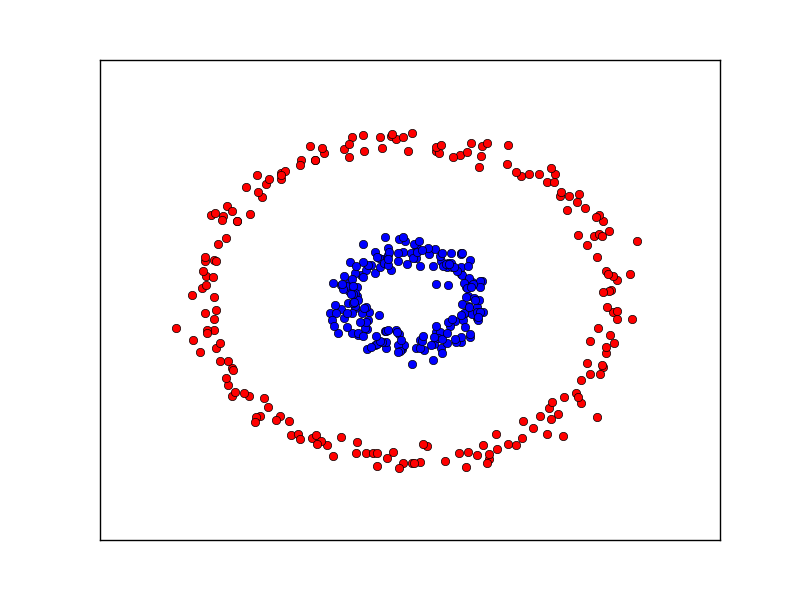
\includegraphics[width=7cm,height=7cm]{figures/ch2_original_data.png}}\hspace{-0.1cm}
\subfigure[An illustration of KPCA feature transformation]{\label{fg:transformated_data}
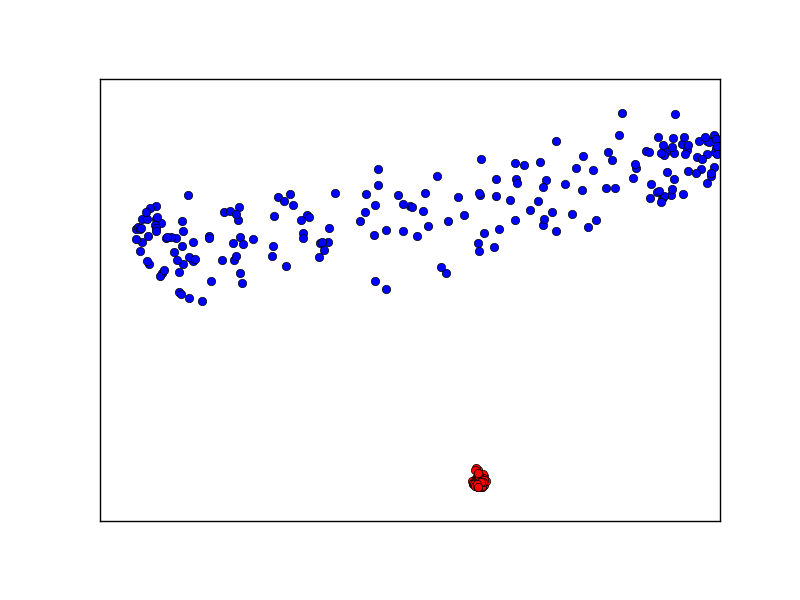
\includegraphics[width=7cm,height=7cm]{figures/ch2_transformated_data.png}}
\caption{Visual kernel mapping}
\end{figure}

\begin{figure}[H]
    \centering
    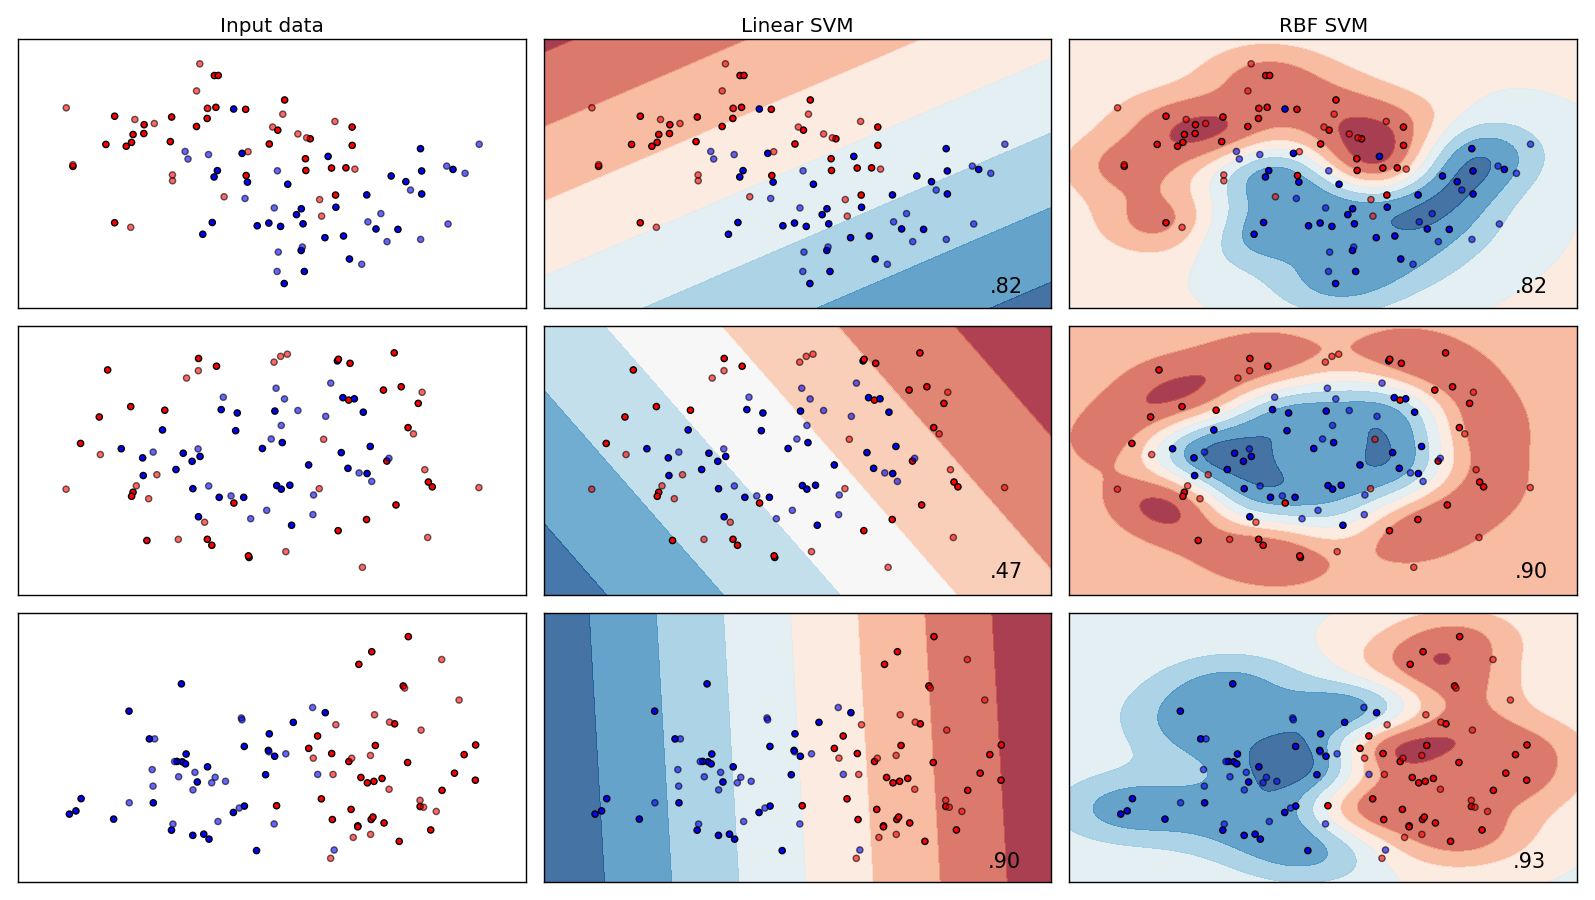
\includegraphics[width=0.8\textwidth]{figures/ch2_SVM_classification_boundary.png}
    \caption{A comparison of linear SVM and nonlinear SVM on synthetic datasets.}
    \label{fig:SVM_boundary}
\end{figure}

For non-linear separable data sets in figure~\ref{fg:orignal_data}, SVM implicitly map the given data set to a linearly separable high dimensional space by using a kernel function $\mathbf{K}<\cdot, \cdot>$, visualization of the KPCA projection figure~\ref{fg:transformated_data}~\cite{jolliffe2002principal}. The kernel SVM be up-grate to a non-linear classifier could be seen in figure~\ref{fig:SVM_boundary}, training points in solid colors and testing points semi-transparent, the lower right shows the classification accuracy on the test set. Since the kernel function is used as an extension of the inner product of the data points, and the size of the product matrix is only related to the data size. The nonlinear expansion obtained by using the kernel function, in the case of small data size, the consume in memory and computation do not result in more complexity. This excellent property makes the application of kernel function very extensive. This section gives a definition of kernel functions and a brief description of the application of kernel functions in support vector machines. Finally, we will discuss how to determine whether a function is a kernel function without constructing a mapping function, which will play a crucial role in deriving quasi-linear kernel functions in later chapters.

\subsection{Definition of Kernel Function}
Let $\mathrm{X}$ be the input space (a subset of the European space $\mathbf{R}^n$ or a discrete set), and $\mathrm{H}$ be the feature space to which the data is projected from the input space through the mapping operator~\cite{scholkopf2001learning}{. For all $x, z \in \mathrm{X}$, if it exits a mapping from $\mathrm{X}$ to $\mathrm{H}$, 
\begin{equation}
\phi(x): \mathrm{X} \to \mathrm{H}
\end{equation}
to ensure that the function $\mathrm{K}<x, z>$ meet the conditions,
\begin{equation}
\mathrm{K}<x, z> = \phi(x)^T\phi(z)
\end{equation}
then called $\mathrm{K}<x, z>$ for the kernel function, $\phi(x)$ for the mapping function.

It can be seen from the definition of the kernel function that the mapping function $\phi(x)$ is usually not explicitly defined in the way of using the kernel function, but directly solves the problem by defining and constructing the kernel function $\mathrm{K}<x,z>$. Review the dual problem of the linear support vector machine deduced in the previous section formula~\ref{eq:2:SVM_dual}. In its optimization goal, only involves the inner product operation $<x_i, x_j>$, therefore it can be replaced by the kernel function $\mathrm{K}<x_i, x_j>$, rewrite the formula~\ref{eq:2:SVM_dual} as:
\begin{equation}\label{eq:2:SVM_dual_Kernel}
\begin{aligned}
\max_{\alpha} ~ &W(\alpha) = \sum_{i=1}^{m}\alpha_i - \frac{1}{2}\sum_{i, j=1}^{m}y_iy_j\alpha_i\alpha_jK<x_i, x_j>\\
s.t. ~ &\alpha_i \geq 0, ~ i = 1,2,...,m\\
&\sum_{i=1}^{m}\alpha_iy_i = 0 
\end{aligned}
\end{equation}

In the same way, the inner product $<x_i, x_j>$ in the classification decision function~\ref{eq:2:SVM_dual_final} can be replaced by the kernel function, thus we can get:
\begin{equation}
\begin{aligned}
f(x) &= sign\Big(\sum_{i=1}^m\alpha_iy_i\phi(x_i)\Big)^T ~ \phi(x) + b \\
      & = \sum_{i=1}^m\alpha_iy_i K<x_i,x> + b
\end{aligned}
\end{equation}

The derivation from the mathematical level explains the kernel function can be used to solve the nonlinear support vector machine approach by solving the solution of linear support vector machine, which is mentioned in the beginning of this section. This technique is often referred to as kernel trick. In actual cases, the choice of the kernel function will greatly affect the final performance of the classifier.

\subsection{Positive Definite Kernel Function}
Since it is necessary to ensure that the designed kernel function is a positive definite kernel function from the viewpoint of theoretical derivation, the sufficient and necessary conditions for positive definite kernel function will be given. The results will provide theoretical evidence for the proof of the quasi-linear kernel function defined in the following section.

Assuming that the kernel function $\mathrm{K}<x,x>: \mathrm{X}\times \mathrm{X} \to \mathrm{R}$ is a symmetric function, then $\mathrm{K}<x, z>$ is a positive definite kernel function if and only if the Gram matrix $\mathrm{K} = [\mathrm{K}<x,z>]_{m\times m}$ corresponding to the kernel function $\mathrm{K}<x,z>$ is a positive definite matrix for any $x_i \in \mathrm{X}, i = 1, 2, \dots, m$.

\section{Quasi-Linear Support Vector Machine}
In this section, we introduce quasi-linear kernel support vector machine theory. In the quasi-linear vector machine model, multiple sets of local linear models are combined with corresponding local threshold functions to form a nonlinear boundary hyperplane~\cite{bo2014quasi, chen2010local}. Different from the conventional method, the quasi-linear support vector machine can obtain the global nonlinear model by integrating all the local models in the kernel space so that the global optimal solution can be obtained only by one global optimization process. The constructed kernel function is called quasi-linear kernel function, which is the key to optimizing the quasi-linear support vector machine by the traditional kernel support vector machine optimization model. In order to construct the quasi-linear kernel function, the common method is to split the local feature space and extract the local information by using the label information to obtain the local threshold function parameters which are needed to construct the quasi-linear kernel function.

\subsection{Mathematical Model of Quasi-Linear Support Vector Machine}
In the case of binary classification problems, suppose we have a training set containing $L$ labeled data points $\{x_i, y_i\}, i=1,2,...,l$, and $x_i\in\mathbf{R}^d$ with a label $y_i \in \{-1,1\}$. First, considering a binary classifier $f(x)$ can be described as:
\begin{equation}
f(x) = g(x), ~~ x\in \mathbf{R}^d \label{eq:2.18}
\end{equation}
where $g(x)$ is a nonlinear function. Applying Taylor expansion to $g(x)$ around the region $x=0$, we can get:
\begin{equation}
f(x) = g(0) + \left(g'(0) + \frac{1}{2}x^Tg''(0)+...\right)x \label{eq:2.19}
\end{equation}
and by defining a vector as:
\begin{equation}
\theta(x) = \left(g'(0) + \frac{1}{2}x^Tg''(0) + ...\right)^T \label{eq:20}
\end{equation}
then we get a regression form of the classifier
\begin{equation}\label{eq:2.21}
f(x)=g(0)+x^T\theta(x)
\end{equation}
where $\theta(x)$ is a vector of unknown functions of x. By introducing an basis function based networks to parameterize the unknown vector $\theta(x)$~\cite{moody1989fast}, we get
\begin{align}
\theta(x)=\sum_{j=1}^{M}\Omega_jR_j(x)+\Omega_0 \label{eq:2.22}\\
g(0)+x^T\Omega_0 = \sum_{j=1}^{M}b_jR_j(x)+b \label{eq:2.23}
\end{align}
\begin{figure}[H]
  \centering
  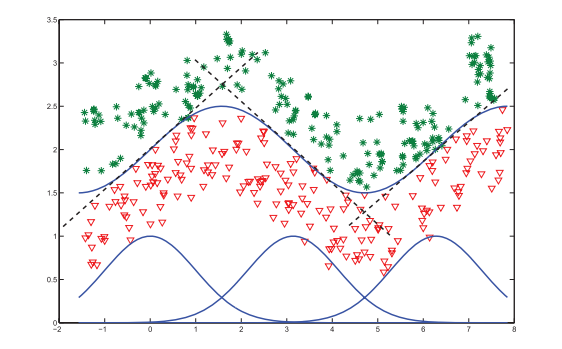
\includegraphics[width=0.7\textwidth]{figures/ch2_visual_QLSVM.png}
  \caption{Multiple local linear classifiers with interpolation for nonlinear separation hyperplane.} \label{fg:visual_QLSVM}
\end{figure}
As a result, we can regard the binary classifier $f(x)$ is constructed by combining with number of $M$ local linear models with local threshold function (see figure \ref{fg:visual_QLSVM})\cite{bo2014quasi}. It can be further defined as follows:
\begin{equation}
f(x)=\sum_{j=1}^{M}\left(\Omega_j^Tx+b_j\right)R_j(x)+b \label{eq:2.24}
\end{equation}
where $\Omega_j(j=1,2,...,M)$ and $b_j(j=1,2,...,M)$ is the parameters of $j$-th local linear classifier, $b$ is the constant parameter and $R_j(x)(j=1,...,M)$ is the local threshold basis functions corresponding each local linear model, it satisfies that $\sum_{j=1}^MR_j(x) = 1$.

Now, we introduce two vectors $\Phi(x)$ and $\Theta(x)$ defined by
\begin{align}
\displaystyle\Phi(x)&=\left[R_1(x),x^TR_1(x),...,R_M(x),x^TR_M(x)\right] \label{eq:2.25}\\
\displaystyle\Theta&=\left[b_1,\Omega_1^T,...,b_M,\Omega_M^T\right]\label{eq:2.26}
\end{align}
the Eq.(\ref{eq:2.22}) can be further expressed as:
\begin{equation}
f(x)=\Theta^T\Phi(x)+b \label{eq:2.27}
\end{equation}

By applying the structural risk minimization principle to the Eq.\ref{eq:2.27}, then a binary classification problem solving process could be described as a QP optimization problem:
\begin{equation}\label{eq:2.28}
\begin{aligned}
&\min_{\Theta,b,\xi_k} J_p = \frac{1}{2}\Theta^T\Theta+C\sum_{k=1}^{N}\xi_k \\ 
s.t. &y_k\left[\Theta^T\Phi(x_k)+b\right]\geq1-\xi_k, \forall k  \\ 
&\xi_k\geq0, \forall k
\end{aligned} 
\end{equation}

Then, by introducing new Lagrange multipliers $(\alpha_k,\nu_k)$, Lagrange function can be constructed in the following forms:
\begin{equation}\label{eq:2.29}
\begin{aligned}
&L(\Theta,b,\xi;\alpha,\nu)=J_p\left(\Theta, \xi\right)\\
&-\sum_{k=1}^{n}\left(\alpha_ky_k\left[\Theta^T\Phi(x)+b\right]-1+\xi_k\right)-\sum_{k=1}^{N}\nu_k\xi_k
\end{aligned}
\end{equation}
Where $\alpha_k\geq0,\nu_k\geq0$. The solution can be given by the saddle point of the Lagrange function as:
\begin{equation}\label{eq:2.30}
\max_{\alpha,\nu}\min_{\Theta,b,\xi}L\left(\Theta,b,\xi;\alpha,\nu\right)
\end{equation}

By applying partial derivative to each parameters:
\begin{equation}\label{eq:2.31}
\left\{ 
\begin{aligned}
&\frac{\partial L}{\partial\Theta}=0 \to \Theta=\sum_{k=1}^{N}\alpha_ky_k\Theta(x_k)\\
&\frac{\partial L}{\partial b}=0 \to \sum_{k=1}^{N}\alpha_ky_k = 0 \\
&\frac{\partial L}{\partial \xi}=0 \to 0 \leq \alpha_k \leq C, ~\forall k \\
\end{aligned}
\right.
\end{equation}

And substitution in formula~\ref{eq:2.30}, we can obtain:
\begin{equation}
\begin{aligned} \label{eq:2.32}
&\max_{\alpha} W(\alpha) = \sum_{k=1}^{l}\alpha_k-\frac{1}{2}\sum_{k,l=1}^{l}\alpha_k\alpha_lK(x_k,x_l) \\ 
s.t. &\sum_{k=1}^{l}\alpha_ky_k=0 \\ 
& 0\leq\alpha_k\leq C, \forall k
\end{aligned}
\end{equation}
where $\mathrm{K}(x_k,x_l)$ is a composite kernel called quasi-linear kernel, defined by
\begin{align} \label{eq:2.33}
K(x_k,x_l)&=\Theta^T(x)\Theta(x)\\ \notag
		       &=(1+x_k^Tx_l)\sum_{j=1}^{M}R_j^T(x_k)R_j(x_l), \forall k,l
\end{align}

From formula~\ref{eq:2.32}, could solve all the parameters in quail-linear kernel SVM which is all $\alpha_k$. So, the final formulation of quasi-linear kernel SVM could write as:
\begin{equation}\label{eq:2.34}
y = sign\left[f(x)\right]
\end{equation}
Where $f(x)$ could write as:
\begin{equation} \label{eq:2.35}
f(x) = \sum_{k=1}^{N}\alpha_ky_kK(x, x_k) + b
\end{equation}
where positive constant $\alpha_k$ is Lagrange multiplier obtained from the QP optimization. The $x_i$ for which $\alpha_k>0$ are called support vectors which contribute to the geometric location of the separation boundary.

\subsection{Quasi-Linear Kernel}
As can be seen from the mathematical formula~\ref{eq:2.33}, quasi-linear kernel function can be seen as an explicit nonlinear mapping of the inner product representation. By adjusting the parameter $M$, that is, changing the number of local linear models, so the mapping performance of quasi-linear kernel function can be adjusted. Furthermore, $K(x_k, x_l) = \sum_{j=1}^{\infty} R_j^T(x_k)R_j^T(x_l)$ is a nonlinear kernel function with the following properties (see figure \ref{fg:QLSVM_M}).

\begin{corollary}
The positive definite of the quasi-linear kernel function: 
Since the quasi-linear kernel function is an inner product representation of an explicit nonlinear mapping, it satisfies the Mercer's theorem, so it is a positive definite kernel function.
\end{corollary}
\begin{corollary}
Modulation function of quasi-linear kernel function: 
The quasi-linear kernel function can adjust the complexity between the linear kernel function and the nonlinear kernel function by adjusting the parameter $M$. When $M = 1$, the quasi-linear kernel function degenerates into a linear function. When $M \to \infty$, the quasi-linear kernel function becomes a product of a linear kernel function and a nonlinear kernel function, so it is a nonlinear kernel function. Figure \ref{fg:QLSVM_M}\cite{bo2014quasi} shows this relationship.
\end{corollary}
\begin{figure}[H]
    \centering
    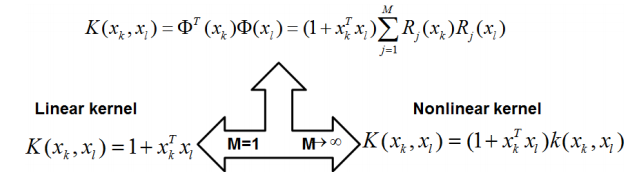
\includegraphics[width=0.8\textwidth]{figures/ch2_QLSVM_numberM.png}
    \caption{Quasi-linear kernel function adjust the number of local linear classifiers.}
    \label{fg:QLSVM_M}
\end{figure}

The quasi-linear kernel function can be constructed by introducing the local threshold basis function $R_j(x)$. When considering a radial basis function (RBF) as the basis function, we have the following expression:
\begin{equation} \label{eq:2.36}
\displaystyle \widetilde R_j(x) = e^{-\frac{(x-\mu_j)^2}{\lambda\sigma_j^2}}, \ 
R_j(x) = \frac{\widetilde R_j(x)}{\sum_{j=1}^{M}\widetilde R_j(x)} 
\end{equation}
Where $\mu_j$ and $\sigma_j$ can be regarded as the center and radius of the threshold basis function, $\lambda$ can adjust the activation range of the threshold basis function in some ability. From the experimental results we can see, when the data were normalized, $\lambda$ value can just be set to 1.

\begin{figure}
    \centering
    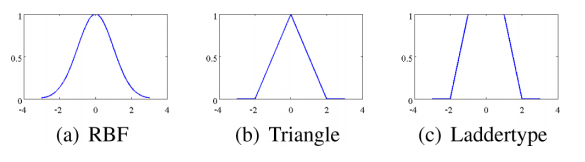
\includegraphics[width=0.8\textwidth]{figures/ch2_basis_function_types.png}
    \caption{Different type of basis threshold functions.}
    \label{fg:basis_function_types}
\end{figure}
Similarly, as shown in figure~\ref{fg:basis_function_types}~\cite{bo2014quasi}, triangular and trapezoidal functions can also be used as a threshold function, the drawback is the lack of smoothness. In the remainder of this thesis, the radial basis function (RBF) is default used as the local threshold basis function for the construction of quasi-linear kernel function.

\subsection{Localization of Feature Space}
From the derivation of the previous sections, it is shown that a quasi-linear kernel function is obtained by multiple local linear models with their corresponding local threshold basis functions. Therefore, before constructing a quasi-linear kernel function, we need to perform a local partition processing of the feature space to obtain the local information to construct each parameter in the threshold basis function.

The clustering technique can automatically decide the partition of local feature space according to the distribution relation of specific training data. B. Zhou uses a two-step approach to determine the final local partitions~\cite{bo2014quasi} (figure~\ref{fg:kmeans_QLSVM}).
\begin{itemize}
\item \textbf{Step 1} According to the boundary detection algorithm, the data points located around the potential hyperplane are selected as the key optimization objects of the local partitioning algorithm, meanwhile, it avoids the extracted local threshold basis function deviates from the potential boundary hyperplane.
\item \textbf{Step 2} Using the modified K-means clustering algorithm to localize the feature space, and avoid local sample unbalance.
\end{itemize}

\begin{figure}[H]
    \centering
    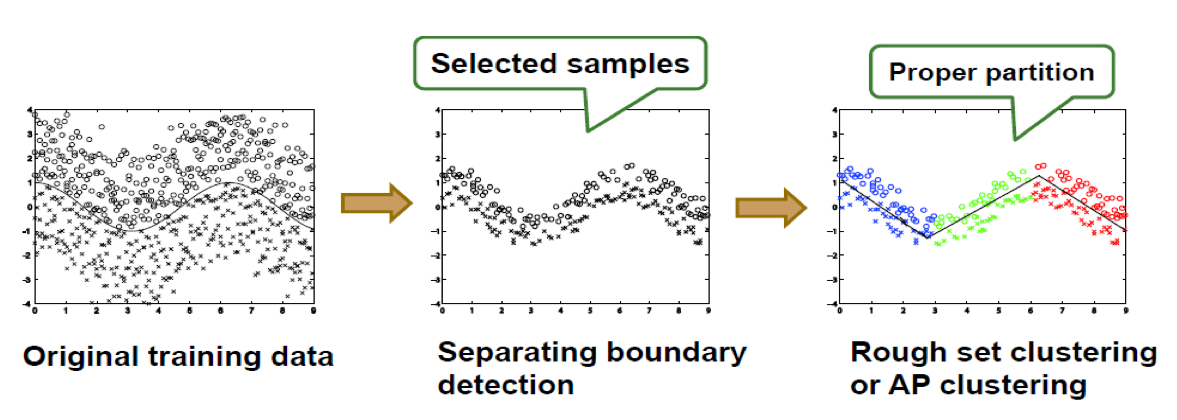
\includegraphics[width=0.8\textwidth]{figures/ch2_kmeans_QLSVM.png}
    \caption{Modified k-means method on an artificial data set.}
    \label{fg:kmeans_QLSVM}
\end{figure}
\begin{figure}[H]
    \centering
    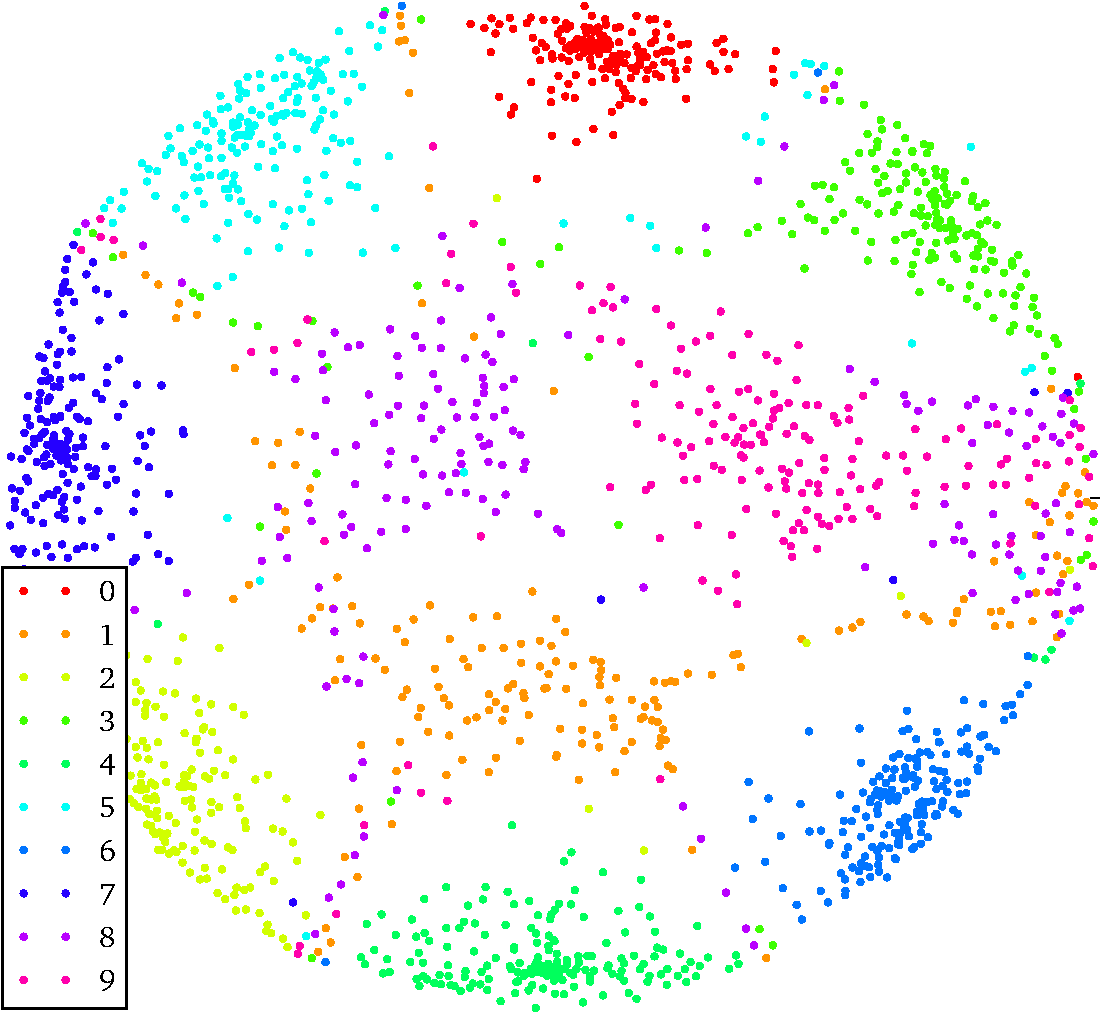
\includegraphics[width=0.5\textwidth]{figures/ch4_proximity_plot.pdf}
    \caption{Proximity plot for a 10-class handwritten digit classification task.}
    \label{fig:proximity-plot}
\end{figure}
But, In the process of construction of quasi-linear kernel function, the unsupervised learning method has a major flaw. Because of the characteristics of the clustering algorithm, it is difficult to deal with the problems like figure~\ref{fig:proximity-plot}.

\chapter{Local Linearity Extraction Based on Samples Space Division}
In the last chapter, the theory and formula derivation of quasi-linear support vector machines are introduced, and the characteristics of quasi-linear kernel functions are illustrated by examples. By analyzing the modified k-means method, some requirements of the constructed a good data-driven quasi-linear kernel functions are summarized.

\begin{enumerate}
\item Partitioned local linear feature space requires the balance of data distribution as much as possible.
\item The center of the threshold function corresponding to partitioned linear feature space should be as close as possible to the potential classification hyperplane.
\item The number of local linear feature spaces should be obtained automatically by the algorithm, rather than artificially pre-specified.
\end{enumerate} 

In this chapter, in order to facilitate the easy understanding, first of all, give an overview of the implementation framework with the help of some illustrative figures, and then discuss in detail of the use of decision trees to identify classification boundaries with local linear partitions. Finally, from the theory of statistical learning, discuss the usefulness and feasibility of extending the decision tree to decision forest, and give a concrete example.

\section{Implementation Framework}
In this part, we give an overview of the implementation framework with the help of some illustrative figures. Some of the implementation details would be introduced in the following sections. Here is the flow:
\begin{enumerate}
\item In order to first detect the nonlinear classification boundary (Remark~\ref{mark:dectect_linear}), we use the fact, even a complexity boundary shape, the small enough local space is approximately linear boundary. According to this idea, we divide the input space of data into small enough space according to some rules, where the data in each subspace can be divided by a linear boundary. Finally, all of the linear boundaries could line up to get a non-linear boundary. In addition, since we already know the label information of all data, the classification result in current subspace can be used as one of the criteria for judging whether or not the division of the subspace is sufficient. Another criterion for determining how to divide the current space is to compute the distance of the data in the space from its center.
\item After solving how to get the local linearity (Remark~\ref{mark:dectect_linear}), we will use ensemble learning method combine with hierarchical cluster algorithm to finally get a set of local linear linearity, in that set, each one includes the final number of local linear classifiers and their function scopes, which is later embedded into the composition of quasi-linear kernel (Remark~\ref{mark:numM}). Finally, we could use valid data to determine which one is the best.
\end{enumerate}
\begin{figure}[H]
    \centering
    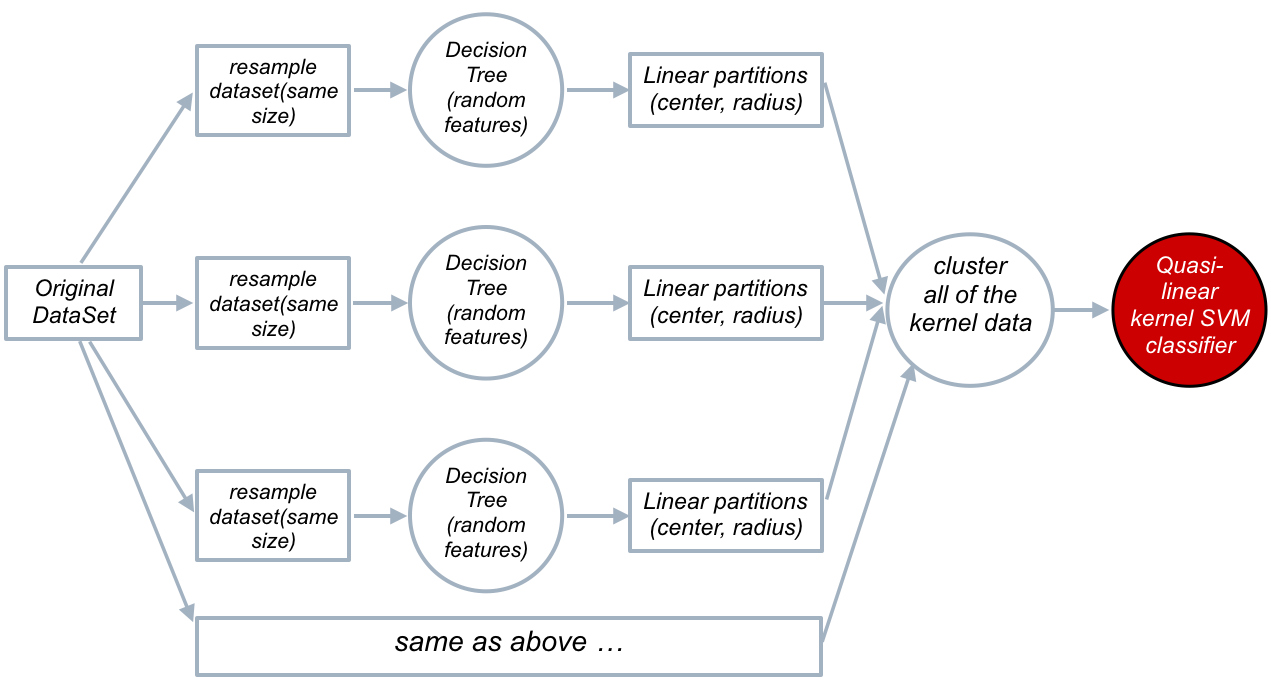
\includegraphics[width=0.9\textwidth]{figures/ch3_RF_framework.png}
    \caption{The framework of the proposed method .}
    \label{fg:RF_frame}
\end{figure}
From the figure \ref{fg:RF_frame} we could see that the basic component of this frame is decision tree, other technique just service as improving the precise of extracted local linearity by the decision tree.

\begin{figure}[H]
\centering
\begin{minipage}{0.55\textwidth}
\hspace{-0.5cm}
\centering
    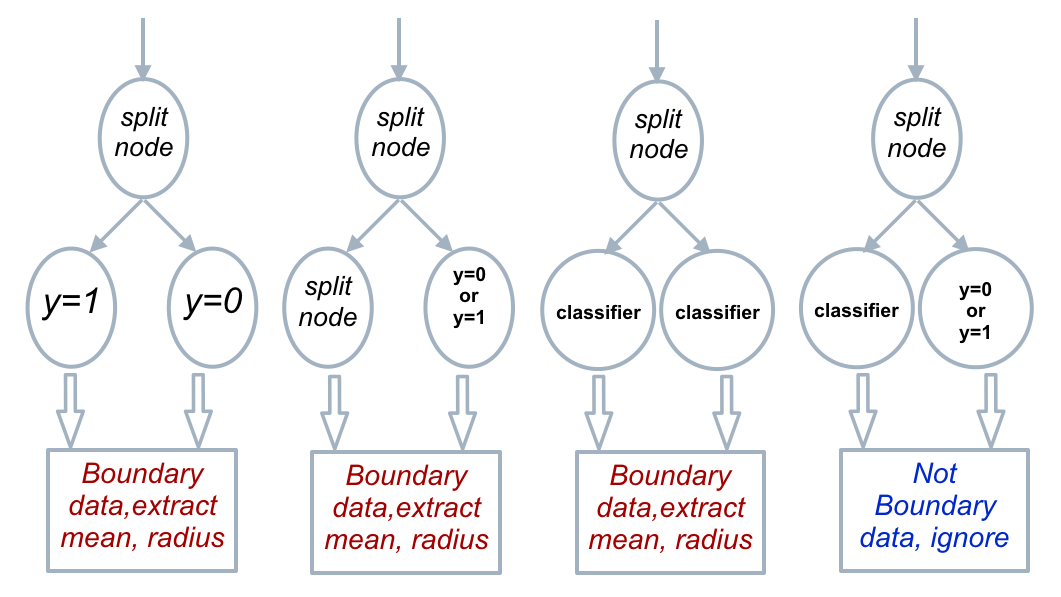
\includegraphics[width=\textwidth]{figures/ch3_extract_condition.png}
    \caption{The extract condition of linear information  in leaf nodes .}
    \label{fg:linear_extract_cond}
\end{minipage}\hfill
\begin{minipage}{0.45\textwidth}
\centering
    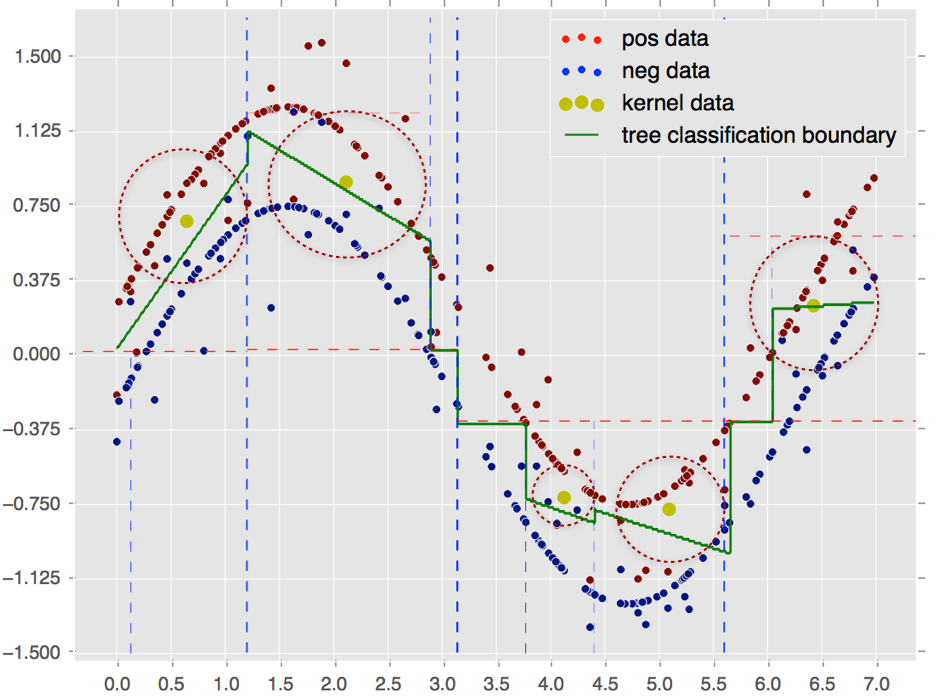
\includegraphics[width=\textwidth]{figures/ch3_extracted_visual.png}
    \caption{The extract linear information at leaf nodes which are linear classifiers.}
    \label{fg:visual_extracted_linear_info}
\end{minipage}
\end{figure}

In figure \ref{fg:linear_extract_cond}, we conclude four conditions when node is split. If the two children sample space is the potential boundary, then the algorithm will calculate the mean and radius corresponding to its sample space.
Followed by this algorithm, figure \ref{fg:visual_extracted_linear_info} shows the final generated tree. In that, the green line is the classification boundary respect to the tree, the red and blue dotted line is corresponding each split feature value, deeper color means closer to the root node. Final, the yellow points are the mean value of the corresponding sample space, the surrounded circle is its radius.
\begin{figure}[H]
    \centering
    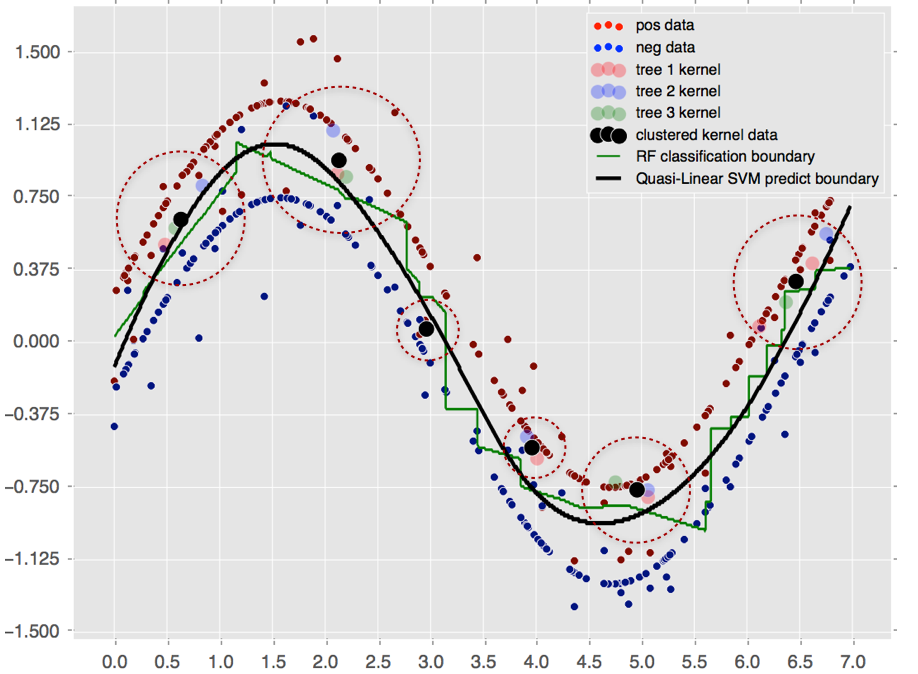
\includegraphics[width=0.8\textwidth]{figures/ch3_QLSVM_byRF.png}
    \caption{The final quasi-linear SVM trained by random forest. }
    \label{fg:QLSVM_byRF}
\end{figure}
Figure~\ref{fg:QLSVM_byRF} give us a final classification boundary of trained quasi-linear kernel SVM which is the black solid line. before getting that line, we cluster all three decision trees' linear information, then get the black points which are the final local linear information. We also could see, compare with the figure~\ref{fg:visual_extracted_linear_info}, the classification boundary combined with three decision trees is more robust and smooth than only one tree.

\begin{figure}[H]
    \centering
    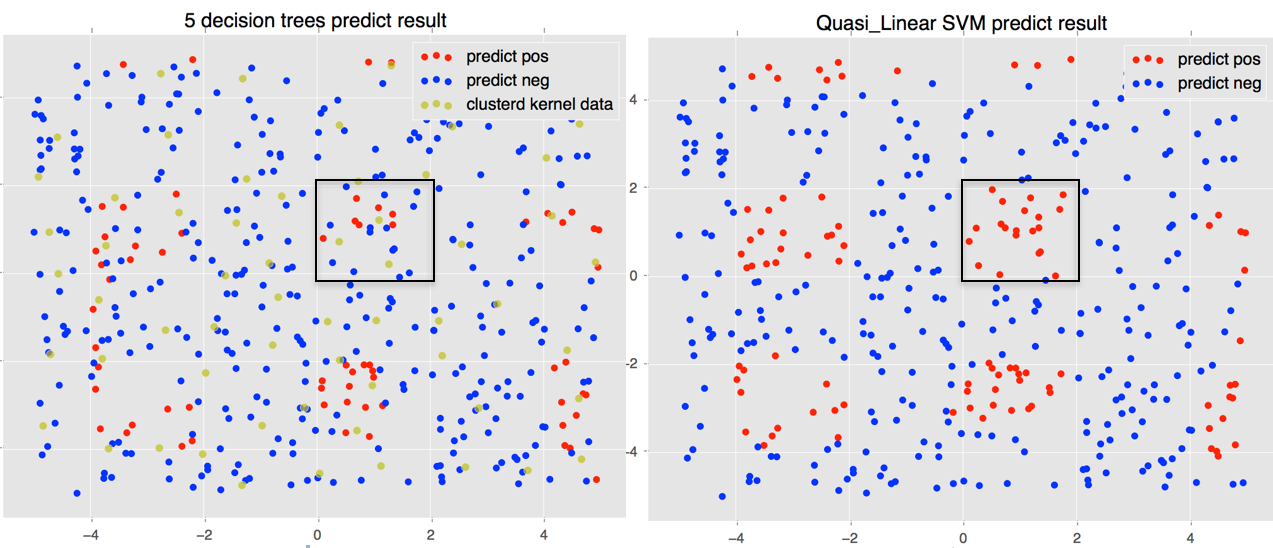
\includegraphics[width=0.9\textwidth]{figures/ch3_RF_QLSVM_compare.png}
    \caption{The final quasi-linear SVM trained by random forest compare with random forest predict result.}
    \label{fg:QLSVM_RF_compare}
\end{figure}
Moreover, in figure \ref{fg:QLSVM_RF_compare}, each block is all same label, this example shows the final quasi-linear SVM trained by random forest has better performance than the random forest predict result. Since the final classification boundary has been globally optimized under the maintenance of the training data geometric shape.

To summary, the whole training frame for quasi-linear kernel SVM can be summarized:
\tikzstyle{startstop} = [rectangle, text width=13cm, minimum height=0.6cm, text centered, draw=black, fill=white!30]
\tikzstyle{io} = [rectangle, text width=13cm, minimum height=0.6cm, text centered, draw=black, fill=white!30]
\tikzstyle{process} = [rectangle, minimum width=5cm, minimum height=0.8cm, text centered, draw=black, fill=white!30]
\tikzstyle{decision} = [rectangle, text width=7cm, minimum height=0.6cm, text centered, draw=black, fill=white!30]
\tikzstyle{arrow} = [thick,->,>=stealth]
\begin{figure}[H]
\centering
\begin{tikzpicture}[node distance=1.2cm]
\node (pro1) [process] {Input training data set, set scale and penalty parameter $\lambda$ and $C$};
\node (pro2) [process, below of =pro1] {Using random forest to train lots of diversity trees};
\node (pro3) [process, below of =pro2] {Each tree calculates a complete local linearity information};
\node (pro4) [process, below of =pro3] {Using cluster algorithm to generate a set of local linearity};
\node (pro5) [process, below of =pro4] {Calculate $R_j(x)$ based on Eq.(\ref{eq:2.36}) using $\mu, \sigma, \lambda$ };
\node (pro6) [process, below of =pro5] {To construct quasi-linear kernel based on Eq.(\ref{eq:2.33})};
\node (pro7) [process, below of =pro6] {Learn all QL SVMs corespond to the quasi-linear kernels with fixed $C$};
\node (pro8) [process, below of =pro7] {Using valid data set to choose the best quasi-linear SVM Eq.(\ref{eq:2.35})};

\draw [arrow](pro1) -- (pro2);
\draw [arrow](pro2) -- (pro3);
\draw [arrow](pro3) -- (pro4);
\draw [arrow](pro4) -- (pro5);
\draw [arrow](pro5) -- (pro6);
\draw [arrow](pro6) -- (pro7);
\draw [arrow](pro7) -- (pro8);
\end{tikzpicture}
\caption{Flow diagram of training process}\label{fg:QLSVM_training_flow}
\end{figure}
In the test stage, the work flow as below:
\begin{figure}[H]
\centering
\begin{tikzpicture}[node distance=1.2cm]
\node (pro1) [process] {Input testing data set, set scale and penalty parameter $\lambda$ and $C$};
\node (pro2) [process, below of=pro1] {Calculate $R_j(x)$ based on Eq.(\ref{eq:2.36}) using the known best local linearity $\mu_j, \sigma_j, M$};
\node (pro3) [process, below of=pro2] {Construct quasi-linear kernel based on Eq.(\ref{eq:2.33})};
\node (pro4) [process, below of=pro3] {Using trained QL SVM to label all the testing data};

\draw [arrow](pro1) -- (pro2);
\draw [arrow](pro2) -- (pro3);
\draw [arrow](pro3) -- (pro4);
\end{tikzpicture}
\caption{Flow diagram of testing process}\label{fg:QLSVM_testing_flow}
\end{figure}

\section{Tree Structured Models}
In this section, we focus on understanding the principle of the decision tree model. The unifying work of Breiman ~\cite{breiman:1984}, later complemented with the work of Quinlan~\cite{quinlan:1993}, have set a series of tree model into a simple and consistent method framework, so, the tree model is gradually widely understood and used. Most importantly, decision trees are the basic component of many moderns and state-of-the-art algorithms, including random forest, which is described later. 

As we will explore in detail later, the success of the decision tree model and the extension model are due to several factors that make it attractive for practical use:
\begin{itemize}
\item Decision trees are a non-parametric model. They can model any complex relationship between the input signal and the output signal without any a prior assumptions.
\item Decision trees can handle multiple types of data, such as discrete or continuous variables, or a mixture of the two.
\item Decision tree actually performs feature selection at the split, which makes the model more robust to irrelevant features or noise variables.
\item Decision trees have the robustness to outliers or errors in labels.
\item Decision trees are very easily to understand its processing.
\end{itemize}

From a geometric point of view, the principle of tree structured models is very simple. It consists of dividing the input space $\mathrm{X}$ into subspaces recursively, and then assigning constant predictive value $\widehat{y}\in\mathrm{Y}$ to all objects $\mathbf{x}$ within each terminal subspace. For the sake of clarity, let us first define the following concepts:
\begin{definition}
A tree is a \emph{directed graph} $G=(V, E)$, in which all edges are from the root node, and any path from root node to the termination node is connected unique.
\end{definition}
\begin{definition}
If there exists an edge from $t_1$ to $t_2$ (i.e., if  $(t_1, t_2)\in E)$ then node $t_1$ is said to be the \emph{parent} of node $t_2$ while node $t_2$ is said to be a \emph{child} of node $t_1$.
\end{definition}
\begin{definition}
In the tree diagram, if a node has one or more child nodes, it is called an internal node; If it has no children node, it is called terminal node or leaf node.
\end{definition}
\begin{definition}
A \emph {binary tree} is a rooted tree in which all internal nodes have up to two children.
\end{definition}

Similarly, the decision tree is also a set of \emph{if-then} rules. The decision eigenvalues of each node in the path from the root node to the leaf node corresponding to the split condition and the class of the leaf node is the conclusion of the rules.

So, in one word, a \textit{tree-structured model} of \textit{decision tree} can be defined as a non-linear transformation $\varphi: X\mapsto Y$, where any node $t$ represents a sub feature space $X_t \subset X$ of the input feature space, with the root node corresponding to input feature space $\mathrm{X}$ itself. Internal nodes $n$ are labeled with a \textit{split} $s_t$ taken from one of the feature space. It divides the feature space $X_t$ that node $t$ represents into disjoint subspaces respectively corresponding to each of its children nodes. 
\begin{algorithm}[H]
Prediction of the output value $\widehat{y} = \varphi(\mathbf{x})$ in a decision tree.
\textnormal{
\begin{algorithmic}[1]\label{algo:prediction}
\Function{Predict}{$\varphi, \mathbf{x}$}
	\State $t = t_0$
	\While{$t$ is not a terminal node}
		\State $t =$ the child node $t'$ of $t$ such that $\mathbf{x} \in X_t$
	\EndWhile
	\State \Return $\widehat{y}_t$
\EndFunction
\end{algorithmic}
}
\end{algorithm}

\begin{figure}[H]
\centering
\subfigure[A decision tree $\varphi$ built for a binary classification problem from an input space $X= {[0, 1]} \times {[0, 1]}$.  ]{\label{fig:3:tree}
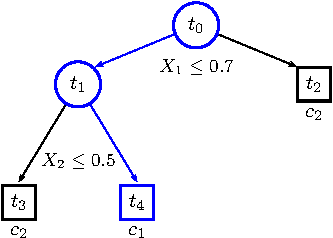
\includegraphics[width=7cm,height=7cm]{figures/ch3_tree.pdf}}\hspace{1cm}
\subfigure[Partition of $X$ induced by the decision tree $\varphi$ into subspaces.]{\label{fig:3:partition}
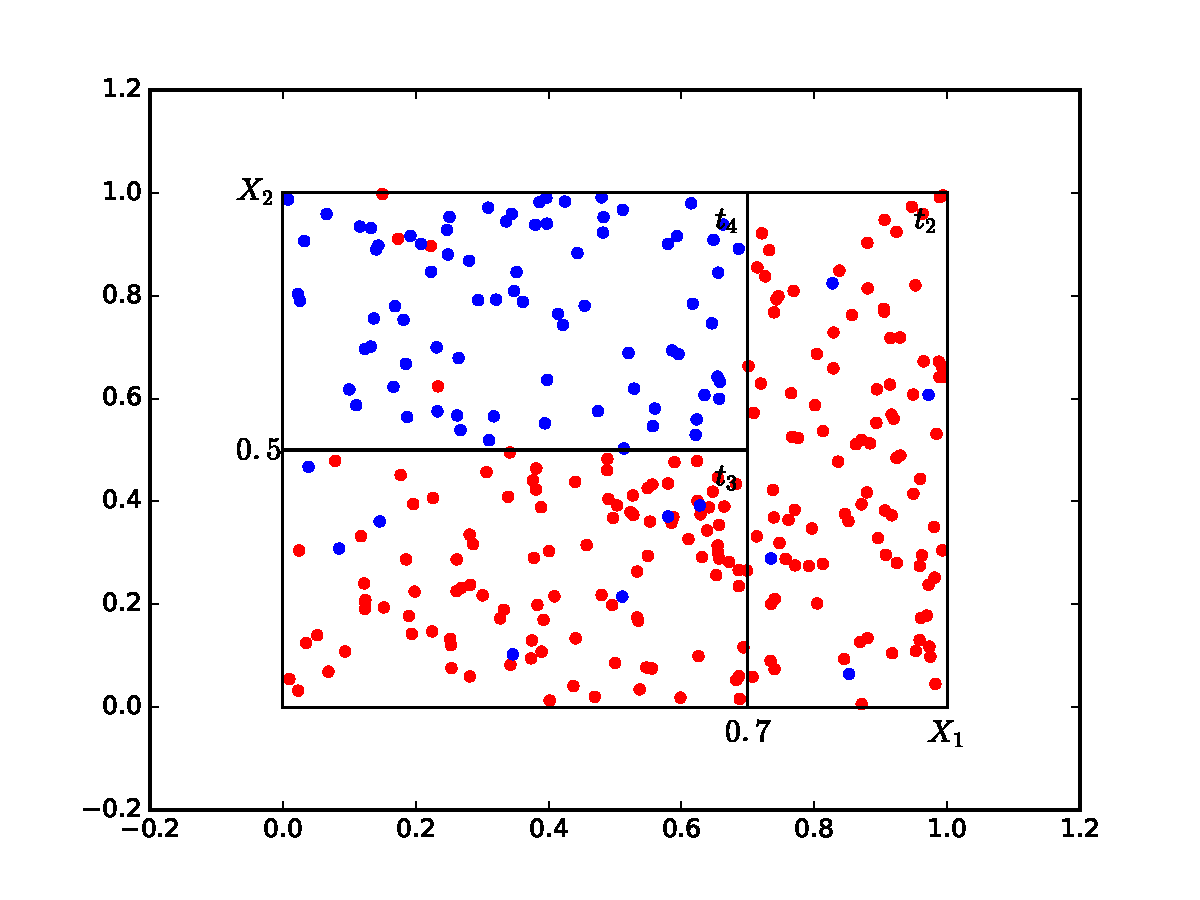
\includegraphics[width=7cm,height=7cm]{figures/ch3_partition.pdf}}
\end{figure}
As an example, figure~\ref{fig:3:tree} illustrate a decision tree $\varphi$ made of five nodes and partitioning the input space $X = X_1 \times X_2 = [0; 1] \times [0; 1]$ for a binary classification problem (where $Y= \{ c_1, c_2 \}$).  Figure~\ref{fig:3:partition} visualize its data space, blue dots correspond to objects of class $c_1$ while red dots correspond to objects of class $c_2$.

\subsection{Splitting Rules}
The decision tree is essentially a set of classification rules derived from the training data set. There may or may not be any decision trees matching the training data set. From another point of view, decision tree model is conditional probability model estimated from the training data set. There are an infinite number of conditional probability models for classes based on feature space partitioning. The conditional probability model we choose should not only fit well the training data but also have a good prediction for the unknown data.

The decision tree learning process also uses the loss function to represent this goal like others. As described below, the loss function of decision tree learning is usually a regularized maximum likelihood function. The decision tree learning strategy is to minimize the loss function as the objective function. When the loss function is determined, the learning problem becomes the problem of choosing the optimal split feature value under the loss function. Since the choosing optimal decision tree from all the possible decision trees is the NP-complete problem, the decision tree learning algorithm actually usually adopts the heuristic method to approximate the optimization problem. Therefore, the resulting decision tree is \emph{sub-optimal}.
Formally, the decrease of impurity of a binary split $s$ is defined as follows:
\begin{definition}\label{def:loss-decrease}
The \emph{loss decrease} of a binary split $s \in S$ dividing node $t$ into
a left node $t_l$ and a right node $t_r$ is
\begin{equation}
\Delta i(s, t) = i(t) - p_l i(t_l) - p_r i(t_r)
\end{equation}
where $p_l$(resp., $p_r$) is the proportion $\tfrac{N_{t_l}}{N_t}$ (resp., $\tfrac{N_{t_r}}{N_t}$)
of learning samples from $L_t$ going to $t_l$ (resp., to $t_l$) and where $N_t$
is the size of the subset $L_t$.
\end{definition}

\begin{figure}[H]
\centering
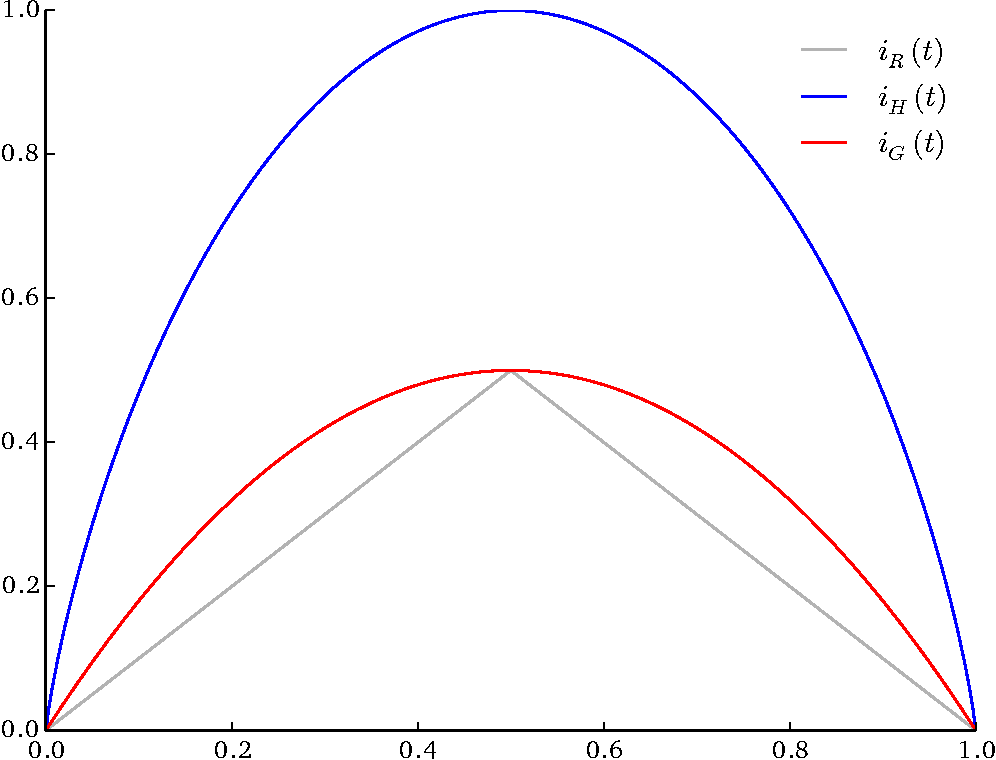
\includegraphics[width=0.6\textwidth]{figures/ch3_impurity_comparison.pdf}
\caption{The relationship in entropy, Gini index and classification error rate}
\label{fig:3:toy:impurity:comparison}
\end{figure}
For purpose of comparison, we illustrate three criteria in loss functions for feature selection, as in figure \ref{fig:3:toy:impurity:comparison}, where $i_R (t)$ is classification error rate, $i_H (t)$ is entropy, $i_G (t)$ is gini index.

Decision tree learning algorithm is a process of usually a recursive selection of optimal features, and according to the selected feature value do train data splitting, so that each sub-data set has the best classification process. This process corresponds to the division of the feature space, also corresponds to the decision tree construction process. This is done until all the training data subsets are classified correctly, or there are no features that can be used to divide.

The process of splitting decision tree is actually the choice of classification features. Important features have a large impact on the outcome of the classification, while irrelevant features have no significant impact on the results. For the decision tree, the feature selection is to decide which feature to use to partition the feature space. 
\begin{figure}[H]
    \centering
    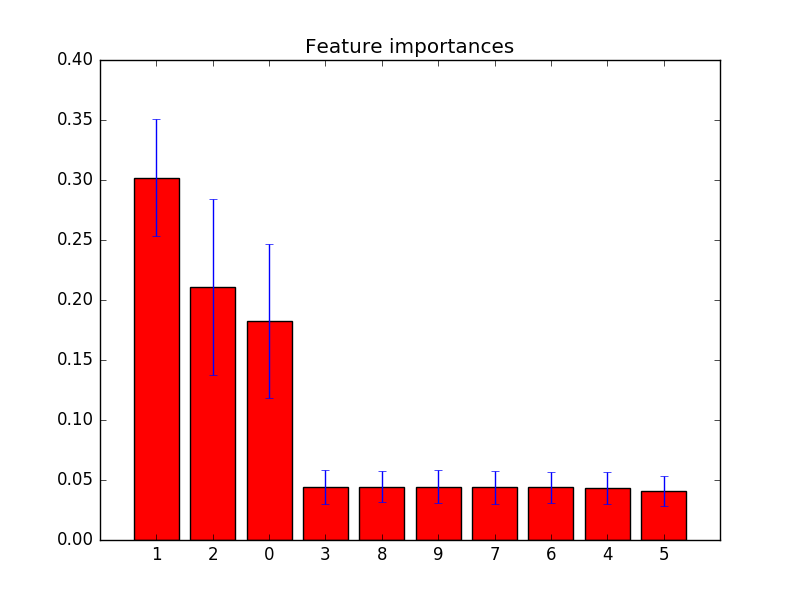
\includegraphics[width=0.7\textwidth]{figures/ch3_feature_importance.png}
    \caption{evaluate the importance of features by random forest.}
    \label{fig:RF_feature_importance}
\end{figure}
Figure~\ref{fig:RF_feature_importance} shows the use of forests of trees to evaluate the importance of features on an artificial classification task. The red bars are the feature importances calculated by random forest (later discuss) along with their inter-trees variability. As expected, the plot suggests that 3 features are informative, while the remaining are not. 

\subsection{Generation of Classification Trees}
In this section, we introduce common decision tree generation algorithms, namely classification and regression tree (CART) model \cite{breiman:1984}. CART is a learning method that outputs the conditional probability distribution of random variable $\mathrm{Y}$ under given input random variable $\mathrm{X}$. CART assumes that the decision tree is a binary tree and the values of the internal node feature are "yes" and "no". Such a decision tree is equivalent to recursively bisecting each feature, dividing the input feature space into finite cells, and confirm the prediction probability distribution on these cells. In our method, the decision tree here based on CART model to modify.

\begin{figure}[H]
\centering
\begin{minipage}{0.55\textwidth}
\hspace{-0.5cm}
\centering
    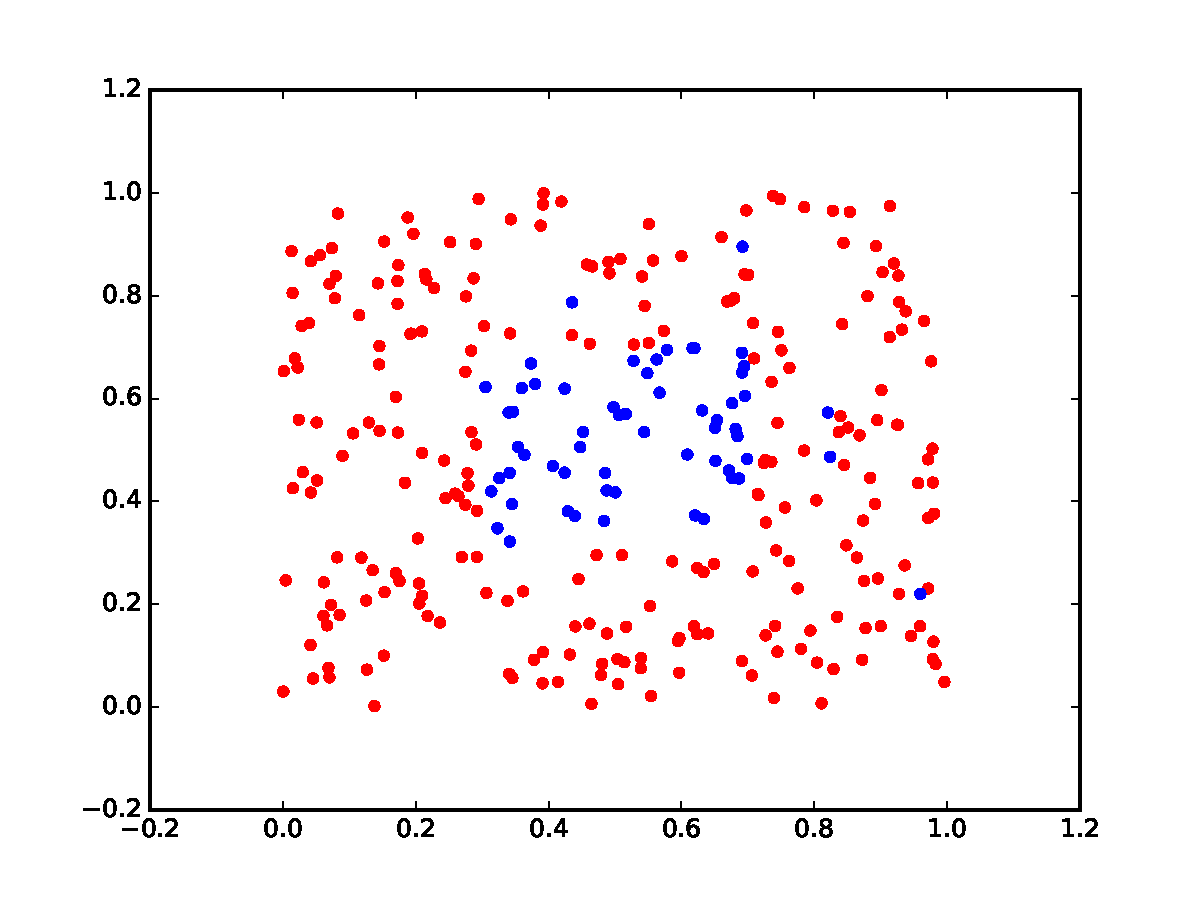
\includegraphics[width=\textwidth]{figures/ch5_learningset.pdf}
    \caption{Binary classification task.}
    \label{fig:5:set}
\end{minipage}\hfill
\begin{minipage}{0.45\textwidth}
\centering
    \includegraphics[scale=0.5]{figures/ch5_tree.pdf}
    \caption{Decision tree learned from Figure~\ref{fig:5:set}.}
    \label{fig:5:tree}
\end{minipage}
\end{figure}

\begin{table}[H]
	\centering
    \small
    \hspace{-0.0cm}
    \begin{tabular}{| l | c c c c c c c c c |}
    \hline
    \texttt{t}    & 0 & 1 & 2 & 3 & 4 & 5 & 6 & 7 & 8 \\
    \hline
    \hline
    \texttt{left\_child} & 1 & -- & 3 & 5 & -- & -- & 7 & -- & -- \\
    \texttt{right\_child} & 2 & -- & 4 & 6 & -- & -- & 8 & -- & -- \\
    \texttt{feature} & 2 & -- & 2 & 1 & -- & -- & 1 & -- & -- \\
    \texttt{threshold} & 0.318 & -- & 0.699 & 0.298 & -- & -- & 0.704 & -- & -- \\
    \texttt{impurity} & 0.315 & 0.020& 0.409 & 0.497 &  0.047 &  0. & 0.4666  & 0. &  0.107 \\
    \texttt{n\_samples} & 300 & 98  & 202 & 120  & 82  & 31  & 89  & 54  & 35\\
    \texttt{value} & 241/59 & 97/1 & 144/58 & 64/56 & 80/2 & 31/0 & 33/56 & 0/54 & 33/2 \\
    \hline
    \end{tabular}
    \caption{Array representation of the decision tree in Figure~\ref{fig:5:tree}.}
    \label{table:tree-array}
\end{table}
As an example, Table~\ref{table:tree-array} shows the array representation of the classification tree which uses Gini index as criteria in loss function.

It can be known that the deeper the tree, the smaller the split feature space of the input feature space is. Obviously, with the exponential growth of leaf nodes, will lead to a dramatic increase in the complexity of the model, finally, the final model will fit the noise data, resulting in over-fitting occurs. Therefore, the decision tree algorithm usually has pruning operations, contains pre-pruning and post-pruning. We will solve this problem by introducing random forest technique in the latter section.

\section{Local Linearity Extraction Based on Decision Tree }
In this section, we will discuss the core idea of this proposed method, namely extract local linearity by decision tree model. In the relative work, Schulter gives us a method how naturally doing a locally linear multivariate regression problem and that random forests nicely fit into this framework~\cite{schulter2015fast}. In their work, they propose a novel regularized objective function optimized during tree growing that operates not only considering the best split feature space but also the best split data space.

Training a single tree involves recursively splitting the training data into disjoint subsets by finding splitting functions for all internal nodes in tree.
\begin{equation} \label{eq3.1}
\sigma(x_j, s^*) = 
\left\{ \begin{aligned}
&L_{t_l} ~ \text{if} ~ r_{s^*}(x_j) < v'_k \\
&L_{t_r} ~ \text{otherwise}
\end{aligned} \right.
\end{equation}
Inspired by them, we propose a loss function considering the division of the input sample space with the classification error rate evaluation criteria, we get the final cost equation as below:
\begin{equation} \label{eq3.2}
E(x_i) = \frac{1}{N}\sum_{n=1}^{N}\left(\Vert y_i - \hat{y_i}\Vert_2^2 + \lambda_1 \cdot \Vert x_i - \bar{X}\Vert_2^2 + \lambda_2 \cdot \Vert x_i - \bar{X}_{y\neg i}\Vert_2^2\right)
\end{equation}
Where, the first term is Mean Square Error (MSE), the second term is the distance of current data from the center of the data space, the third term is the distance of current data away from the opposite label data center.

The intuition of the 2,3-th terms is that we not only require to put samples in a leaf node that have right predicted label $\hat{y_i}$, we also want those samples themselves (i.e. $x_i$) to be cluster (compactness) as a simple shape so that these data could fall into the same leaf node, which potentially eases the task for the linear classification model $m_l(x_i)$ in the leaf.
By the way, the 2,3-th terms in this formula are from Pearson Correlation, which is used to calculate the similarity of two vectors.
\begin{align}
Corr(x, y) &=  \frac{\sum_i(x_i - \bar{x})(y_i - \bar{y})}{\sqrt{\sum(x_i-\bar{x})^2}\sqrt{\sum(y_i - \bar{y})^2}}
&= \frac{<x - \bar{x}, y - \bar{y}>}{||x-\bar{x}||||y- \bar{y}||}
&= CosSim(x-\bar{x}, y- \bar{y}) 
\end{align}

After fixing the best split $\sigma(\cdot)$ according to Eq~\ref{eq3.2}, the data in the current node is split and forwarded to the left and right children respectively. Growing continues until one of the stopping criteria is met and the final leaf nodes are created. In our method, The needed $\mu$ and $\lambda$ in Eq.(\ref{eq:2.36}) are calculated in the datasets in the corresponding leaf node which is the boundary data, specific, we calculate the mean value and standard deviation as the $\mu$ and $\lambda$. For preciser result, this method could be improved.

\begin{figure}[H]
    \centering
    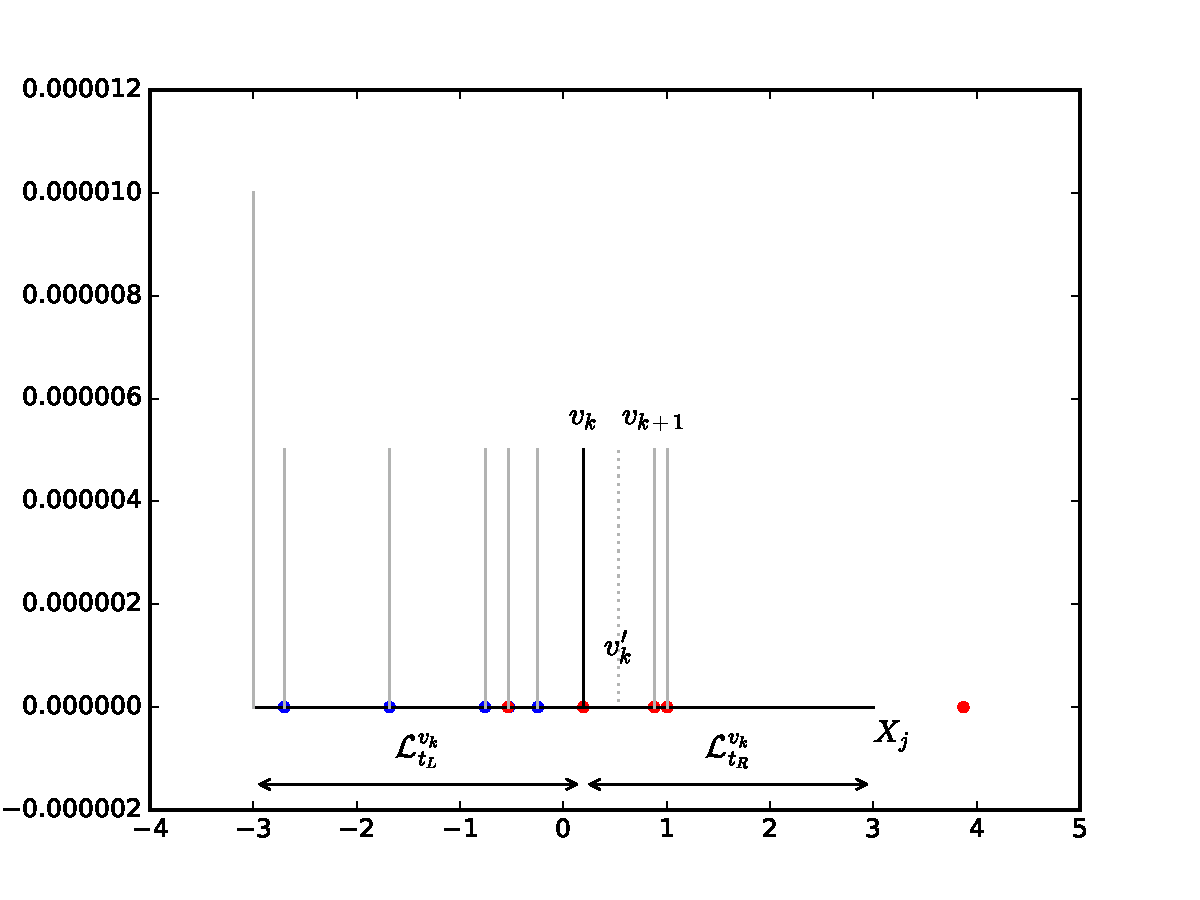
\includegraphics[width=0.9\textwidth]{figures/ch3_split_ordered.pdf}
    \caption{Binary partitions of $L_t$ on the ordered variable $X_j$. Setting the decision threshold $v$ to any value in $[v_k,v_{k+1}]$.}
    \label{fig:3:split_ordered}
\end{figure}
The important thing here is that assuming distinct input values for all $\mathrm{N_t}$ node samples, the number of partitions of ${L_t}$ into $k$ non-empty subsets is given by the Stirling number of the second kind~\cite{knuth1992problem}:
\begin{equation}
S(N_t, k) = \frac{1}{k!}\sum_{j=0}^k(-1)^{k-j} {k\choose j} j^{N_t},
\end{equation} 
which reduces to $2^{N_t-1}-1$ for binary partitions. Given the exponential growth in the number of partitions, the naive strategy of enumerating all partitions and picking the best of them is often computationally intractable. For this reason, in our method, we will choose almost 66\% percent of continuous feature values as candidate split point. We usually assumes that $s^*$ is a good enough approximation, lives in a family $s^* \subseteq {S}$ of candidate splits of restricted structure (figure~\ref{fig:3:split_ordered}). 

To summary, we lead to the following procedure:
\begin{algorithm}[H]
Find the best split $s^*$ that partitions $L_t$.
\textnormal{
\begin{algorithmic}[1]\label{algo:findsplit}
\Function{FindBestSplit}{$L_t$}
    \State $\Delta = -\infty$
    \For{$j=1, \dots, p$}
        \State Find the best binary split $s^*_j$ defined on $X_j$ \label{algo:best-split-line4}
        \If{$\Delta i(s^*_j, t) > \Delta$}
            \State $\Delta = \Delta i(s^*_j, t)$
            \State $s^* = s^*_j$
        \EndIf
    \EndFor
    \State \Return $s^*$
\EndFunction
\end{algorithmic}
}
\end{algorithm}


\section{A Random Forest Framework}
From the previous section, we have explained that based on CART algorithm, by using our new loss function, we could use it to extract local linearity (figure~\ref{fg:visual_extracted_linear_info}). However, in order to ensure the generalization performance of the model, usually, the pruning operation must be carried out during the training process. But, we have a better way to fix this problem by naturally introduce decision forest. We say the decision forest is based on the ensemble learning theory. Briefly, the benefits are obvious:
\begin{itemize}
\item First, the generalization performance of the whole model is better.
\item Secondly, no longer needs worry about the over-fitting problem, means we do not need prune operations.
\end{itemize} 

Thus, the linear partition based on the combination of all of the decision trees will ensure that the constructed quasi-linear kernel function has more precise data shape information. So, the final trained QL-SVM could improve its performance.

This section is organized as follows: first, introduce the basic theory of ensemble learning method, explain its characteristics and the place need to pay attention to which it is implemented; Then introduce Random Forest learning framework; finally, we discuss how to use the random forest~\cite{breiman2001random} to extract the segmentation linearity of the input sample with clustering algorithm.

\subsection{Ensemble Learning Methods}
Ensemble learning is accomplished through the construction and integration of multiple learners to complete the learning task, sometimes called multi-classifier system. The general structure of ensemble learning: 
\begin{enumerate}
\item Generate a group of individual learners and then combine them with some strategy, in which the individual learner is usually an existing learning algorithm, such as CART. 
\item The integrated individual learners are the same type, such as all of the decision tree, this integration is called homogeneous. Relatively, if the individual learners are different, called as heterogeneous.
\end{enumerate}

Ensemble learning usually could obtain better generalization performance than the single learner, especially when the individual learner is a weak learner. In addition, when strong learners are used, generally less individual learner integration can achieve better generalization performance.
\begin{equation} \label{eq:3.6}
H(x) =\mathrm{sign} \left(\sum_{i=1}^Th_i(x)\right)
\end{equation}
Eq.~\ref{eq:3.6} says that the ensemble method combines a number of T of basis classifiers with a simple voting method, if more than half of the basis classifiers are correct, then the integration classification is correct.

Assuming that the error rates of the basis classifiers are independent of each other, the Hoeffding inequality shows that the integrated learning error rate is:
\begin{equation} \label{eq:3.7}
\begin{aligned}
P(H(x)  \neq f(x)) &= \sum_{k=0}^{\lfloor T/2 \rfloor}
\left(\!\begin{array}{c}
T \\ k
\end{array}
\!\right)
(1-\epsilon)^k\epsilon^{T-k} \\
& \leq \mathrm{exp}\left(-\frac{1}{2}T(1-2\epsilon)^2\right)
\end{aligned}
\end{equation}
From formula~\ref{eq:3.7} we could see that with the increase in the number of base learners, the ensemble error rate will exponentially decline, and ultimately tend to zero.

However, the individual learners must match with some requirements. if expected to get good training result, it is necessary that all of the base learners as different as possible while they have somehow good performance. In fact, if all the base learner input data are the same, then the above request is very contradictory, so the core research of ensemble learning is focused on to solve this problem (\cite{krogh1995neural,breiman1996bagging,kohavi1996bias}). Finally, there are two types of combination strategies: average method, "learning method".

\begin{remark}{Ambiguity decomposition}
For prediction averaging, as defined in Equation~\ref{eq:3.6}, the \textit{ambiguity decomposition} guarantees the generalization error of the ensemble to be lower than the average generalization error of its constituents~\cite{krogh1995neural}. Formally, the ambiguity decomposition states that
\end{remark}
\begin{equation} \label{eq:3.8}
E = \overline{E} - \overline{A}
\end{equation}
where $\overline{E} = \sum_{i=1}^Tw_iE_i$ and $\overline{A} = \sum_{i=1}^Tw_iA_i$,
the first term is the average generalization error of the individual models, the second term is the ensemble ambiguity and corresponds to the variance of the individual predictions around the prediction of the ensemble. Since $\overline{A}$ is non-negative, the generalization error of the ensemble is therefore smaller than the average generalization error of its constituents.
Formula \ref{eq:3.8} clearly points out that the higher the accuracy of individual learners, the greater the diversity, the better integration performance could be achieved. 

\subsection{Random Forest}
One of the ensemble models, called Random Forest, is a parallel model, in which there is no dependency between individual learners, and learning tasks can be performed at the same time~\cite{breiman2001random}. As we can see from the previous subsection, for the strong generalization performance, the individual learners in the ensemble should be as independent as possible. Although pure independence can not be achieved, we can try to make the base learner as different as possible. Random forest (RF), a word summary, is the combination of many diversity decision trees. It improves the diversity of the trees in the following way:
\begin{itemize}
\item The input data is adjusted first, using the Bagging method~\cite{breiman1996bagging}, which is based on bootstrap sampling. Specifically, the flow is as follows: for a given data set containing \textit{m} samples, we first randomly draw one from it into the sample set, and then put the sample back to the initial data set, so that in the next sampling process the same one still has a chance to be chosen. Now, after \textit{m} times re-sampling process, we can get a sample set with \textit{m} samples, in which some samples in the initial training set appear many times in the sampling set, while others never appear. From formula~\ref{eq:3.6}, about 63.2\% of the samples in the initial training set appear in the sampling set. In this way, we can get a number of \textit{T} sample sets with each has \textit{m} training samples. Now, we could train a decision tree based on each sample set and then combine these decision trees.
\begin{equation} \label{eq:3.9}
\lim_{m \mapsto \infty} \left(1 - \frac{1}{m}\right)^m \mapsto \frac{1}{e} \approx 0.368
\end{equation}
\item Random forest introduces stochastic feature selection in the training process of the decision tree. In the traditional decision tree, the optimal feature is selected in the feature set of the current node. In RF, at the current node, firstly, a subset of $k$ features is selected at random, and then an optimal feature is selected from the subset for splitting process. Here, the parameter $k$ controls the degree of randomness: if $k = d$, the construction of the decision tree is the same as that of the traditional decision tree; if $k = 1$, then a feature is chosen randomly for splitting; in general, The recommended value $k = log_2d$.
\end{itemize}

For simple analysis, If the computational complexity of a single decision tree is $O (m)$, $O(s)$ is the complexity of the sampling and integration process, So train a random forest is almost $T(O(m)+O(s))$, with the same order of complexity compares with direct use of a decision tree. Therefore, the random forest is simple, easy to implement, computational overhead is small, but it shows a strong performance in a lot of real tasks.

\begin{figure}[H]
    \centering
    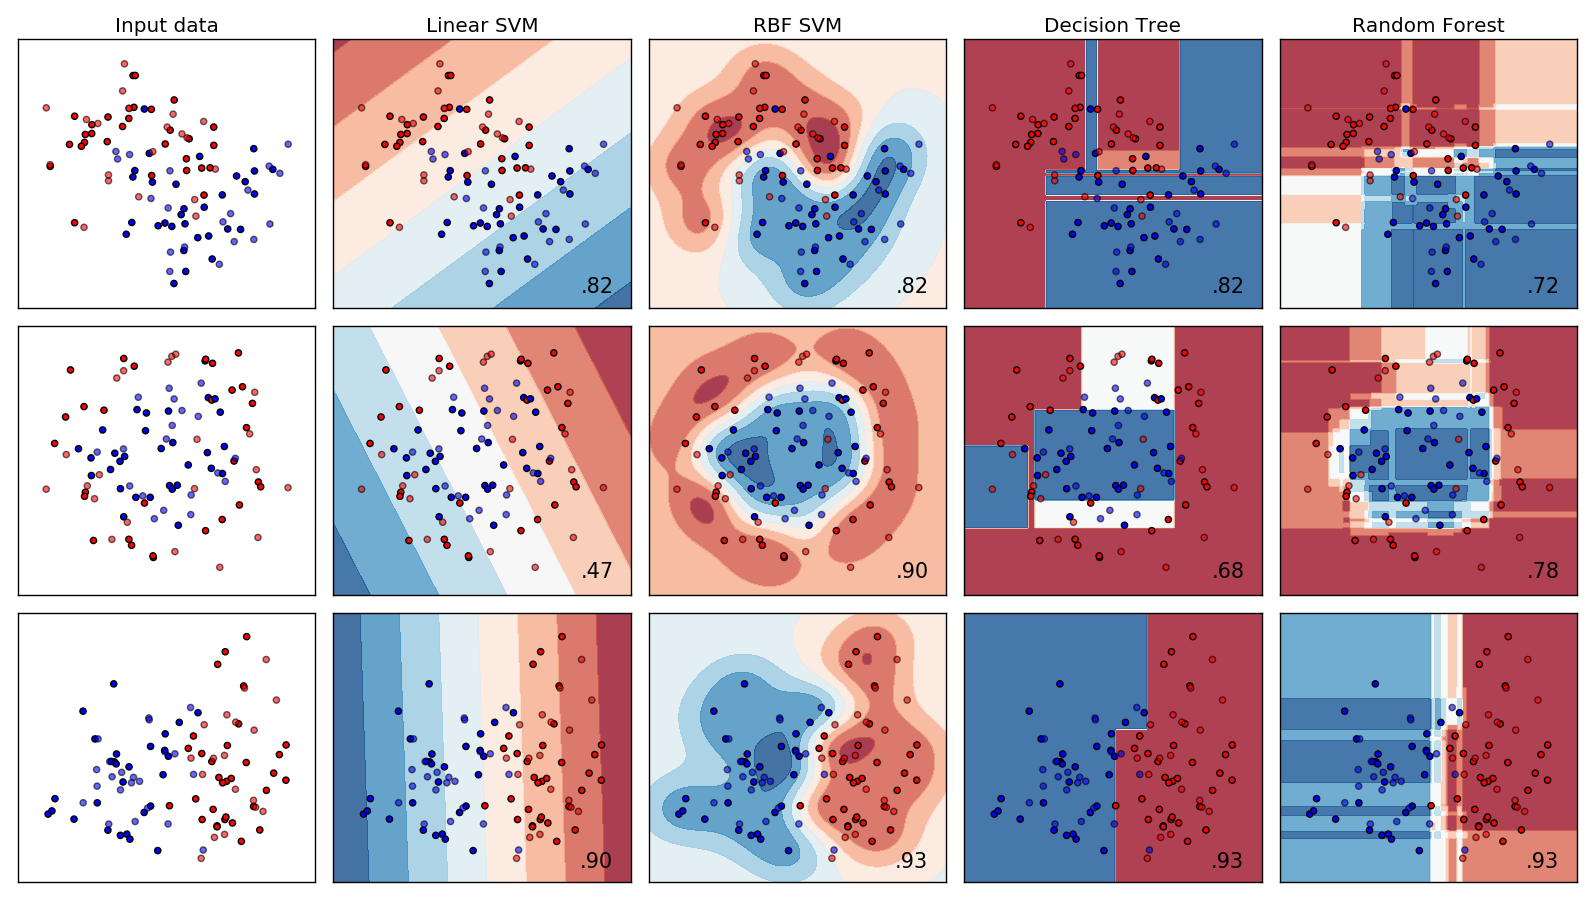
\includegraphics[width=0.9\textwidth]{figures/ch3_SVM_RF_boundary.png}
    \caption{A comparison of classification boundaries of a several classifiers on synthetic datasets.}
    \label{fig:SVM_RF_boundary}
\end{figure}
Figure~\ref{fig:SVM_RF_boundary} is a comparison of a several classifiers on synthetic datasets. The plots show training points in solid colors and testing points semi-transparent. The lower right shows the classification accuracy on the test set. From figure \ref{fig:SVM_RF_boundary} we can conclude that RF could use combination of all classification boundaries corresponding each decision tree get a good non-linear separation boundary. 

To sum up how to enhance diversity. The general idea is to introduce randomness in the learning process. The common ways are to disturb the data samples, input features, output results or model parameters. In RF, we use the data disturb and features disturb. 
\begin{itemize}
\item The data disturb makes only about two-thirds of the original training samples appear in the training samples of each tree, and some of the samples are repetitive. From the perspective of the boosting learning method, we can say that this is equivalent to re-weighting the input samples. The weight of the data does not appear as 0, appeared once as 1, appeared twice as 2, and so on.
\item RF also uses the features disturb, we know that the split process is actually a process of feature selection, and in RF each time only considers the subset of features. So with a deeper understanding, the splitting process of the decision tree first maps the feature space to some sub-feature space, next selects one.
\item Furthermore, if the parameters of each tree in the random forest are mixed with randomness, this will make the prediction hypothesis space of each tree become more different, namely, the model complexity of the each tree is quite different.
\end{itemize}

\subsection{Cluster Local Linear Partitions}
In this paper, each decision tree will get a complete set of local linear information, but the cause of the performance of the model itself, this set of information is not accurate. However, it is sure that this set can express the approximate geometric information of the training data. In order to obtain more accurate local linear information, firstly we obtain several different sets of local linear information by random forest algorithm which uses lots of diversity decision trees; next, to obtain a set of reliable local linear information, hierarchical clustering algorithm is used, which can ensure that the extracted geometric information is not lost during the clustering process.

In this section, we first give the hierarchical clustering algorithm's diagram, explain its working principle, and then give the local linear partitions graph after clustering.

\begin{figure}[H]
    \centering
    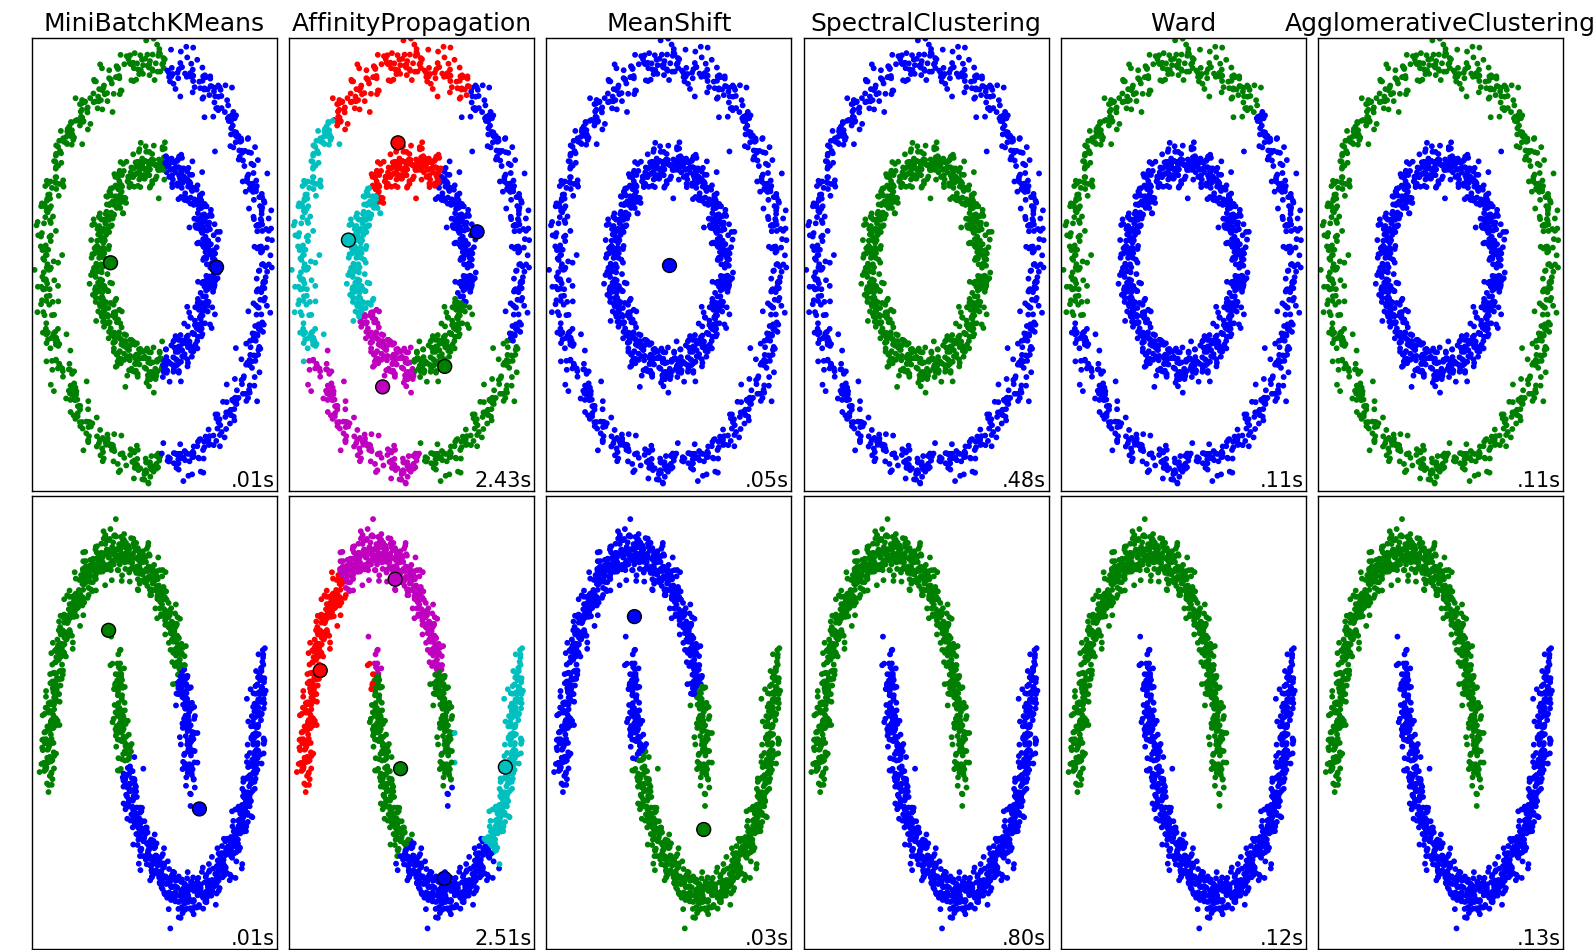
\includegraphics[width=0.9\textwidth]{figures/ch3_compare_cluster.png}
    \caption{Show characteristics of different clustering algorithms. }
    \label{fig:cluster_comparision}
\end{figure}
Figure~\ref{fig:cluster_comparision} aims at showing characteristics of different clustering algorithms. We can see that spectral clustering and agglomerative clustering could keep the data structure when doing clustering operation. So, In our method, we use agglomerative cluster do the local linear information cluster.

\begin{figure}[H]
    \centering
    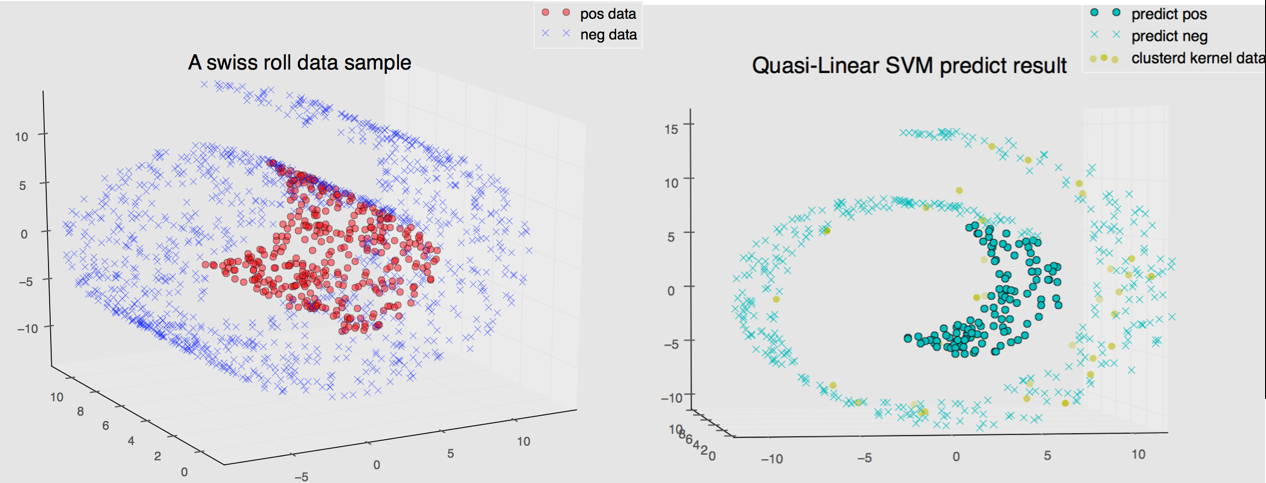
\includegraphics[width=0.9\textwidth]{figures/ch3_cluster_linear_info.png}
    \caption{Proposed method handle with non-linear data set}
    \label{fig:cluster_linear_info}
\end{figure}
From figure~\ref{fig:cluster_linear_info}, we can know that by keeping geometric information during local linearity cluster process, final trained quasi-linear SVM still a good non-linear classifier, so that could handle with non-linear data set like figure~\ref{fig:proximity-plot}.

\begin{figure}[H]
    \centering
    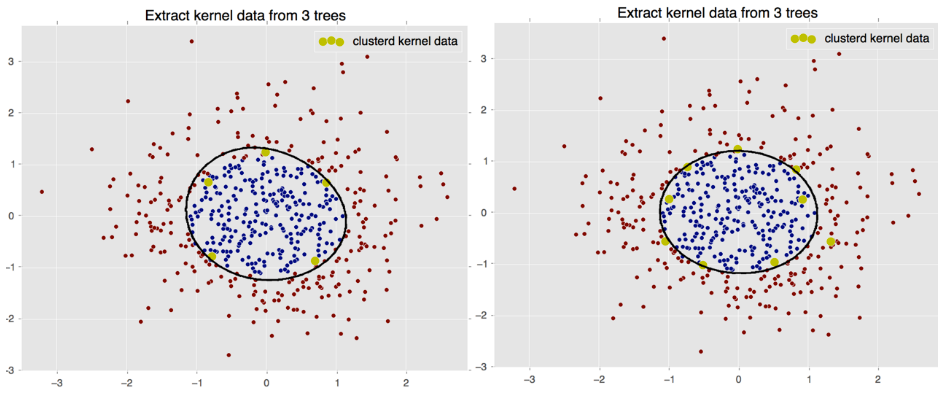
\includegraphics[width=0.9\textwidth]{figures/ch3_cluster_M_number.png}
    \caption{Proposed method choose variable number of local linear classifiers after training random forest.}
    \label{fig:cluster_M_number}
\end{figure}
From figure~\ref{fig:cluster_M_number}, we can say that our method is flexible enough when choose the number of local linear classifiers. This property is very import for constructed quasi-linear kernel performance (from Remark~\ref{mark:numM}).

\chapter{Experiments}

In this section, we evaluate our algorithm on real-world data sets, the results as shown in the following figures and tables. In our experiments, the LIBSVM tool developed by Chang and Lin~\cite{chang2011libsvm} is taken as a basis and all experiments are conducted on a Windows 7 machine with a $1.8GHz$ CPU and $8.0GB$ of RAM.

\section{Evaluation Metrics}
Since we focus on the improvement of classifier performance on binary classification, for data sets containing more than two classes, we use one-versus-all strategy to transform a multi-class problem to multiple binary classification problems. In addition, we use L2 normalization method to pre-process data.

In section \ref{UCI}, we use $accuracy$ as the metric to examine the performance comparison between the quasi-linear kernel and other kernels and Random Forest. In section~\ref{Yeast}, we have a data sets characterized by high-noise, in order to provide a comparable result, these three indicators are specifically designed for binary classification problems to be used, which is called $precision$, $recall$ and $F-1$ score. Conceptually, the $precision$ represents the proportion of the positive samples to the samples of all the positive samples. The $recall$ represents the proportion of the positive samples to the original samples. The four evaluation indicators can be calculated by the following form:
\begin{equation}
\begin{aligned}
accuracy &= \frac{TN+TP}{TN+TP+FN+FP} \\
precision &= \frac{TP}{TP + FP} \\
recall &= \frac{TP}{TP + FN} \\
F-1 &=\frac{2 \times precision \times recall}{Precision + recall} 
\end{aligned}
\end{equation}
Where TP represents the number of positive class samples correctly judged as a positive class; FP represents the number of negative class samples judged as a positive class by mistake; FN represents the number of positive class samples that are wrongly judged as negative class. 

\section{UCI Data Set}\label{UCI}
In order to compare the classification accuracy of each algorithm on the actual data set, this section compares and summarizes the performance of each algorithm using 7 widely used data set from the UCI machine learning database~\cite{asuncion2007uci}. In Table \ref{table:1.1}, we summarize the characteristics of the selected data sets such as the features, the sizes,  the number of positive and negative samples. 

\begin{table}[H]
\renewcommand\arraystretch{1.2}
\centering \caption{Description of the data sets\label{table:1.1}}
\begin{tabular}{c|c|c|c|c}
\hline
data sets & features & Positive & Negative & Total \\
 \hline\hline
Breast~\cite{wolberg1990multisurface} & 10 & 458 & 241 & 699 \\
Glass & 9 & 70 & 144 & 214 \\
banknote & 4 & 610 & 762 & 1372 \\
Yeast-MIT~\cite{horton1996probabilistic} & 8 & 244 & 1242 & 1486 \\
Yeast-NUC & 8 & 430 & 1056 & 1486 \\
Yeast-CYT & 8 & 464 & 1022 & 1486 \\
Yeast-ME3 & 8 & 163 & 1323 & 1486 \\
Sonar~\cite{gorman1988analysis} & 60 & 97 & 111 & 208 \\
Arrhythmia~\cite{guvenir1997supervised} & 279 & 245 & 207 & 452 \\
Haberman & 3 & 225 & 81 & 306 \\
\hline
\end{tabular}
\end{table}

In the tree parameter selection, we set tree number is 10, the random feature size is $log_2d$, the split threshold is linear classification error less than 5\%,  min samples in the leaf is 10. For the SVM relative parameter selection, we set $C\in\{0.1,0.5,1,5,10,20,50\}$ and $\gamma\in\{1\}$ for the quasi-linear SVM, and using a 3-fold cross-validation to train each quasi-linear SVM in the set kernels of each one has a different number of local linear classifiers, then choose the best one. On the other hand, a 3-fold cross-validation is used to estimate parameters like $\gamma\in\{0.1,0.5,1,5\}$ for SVM with RBF kernel and $C\in\{0.1,0.5,1,5,10,20,50\}$ for SVM with RBF and linear kernels. For each data set, we randomly split the data set into two halves, one-half for training, the other for testing. Table \ref{table:1.2} summarizes the mean accuracies and the standard deviations. The result is the average performance of 50 times of random trials. 

In Table \ref{table:1.2}, it can be seen that the quasi-linear kernel function overcomes the performance of linear kernel function and the RBF kernel function on the most data sets, even though cross-validation of the hyperparameters is not performed (with the choice of a broader hyperparameter range, it is possible to make RBF kernel function to achieve better performance). This means that although the quasi-linear kernel function is designed to substitute RBF kernel function as a nonlinear model when the RBF kernel function is over-fitted, an effective potential boundary can be obtained by accurately designing the local threshold basis function, this prior knowledge can make quasi-linear kernel function more powerful than the traditional widely used kernel functions. Moreover, RF trained classification boundary is also a robust one, although it is not optimized in a global view.

\begin{table}[H]
\renewcommand\arraystretch{1.2}
\centering \caption{The classification accuracies of SVM with different kernels and RF\label{table:1.2}}
\begin{tabular}{ c | c | c | c | c}
\hline
data sets & Linear Kernel& RBF Kernel& Quasi-Linear Kernel & Random Forest\\
 \hline\hline
Breast & 87.6103$\pm$0.0132 & 89.0591$\pm$0.0139 & 89.1434$\pm$0.0027 & \textbf{92.8236$\pm$0.0465} \\
Glass & 74.4723$\pm$0.0424 & 78.8403$\pm$0.0366 & \textbf{81.3139$\pm$0.0680} & 79.4412$\pm$0.0472\\
banknote & 98.7812$\pm$0.0032 & 99.8201$\pm$0.0017 & \textbf{99.8532$\pm$0.0025}& 99.2782$\pm$0.0045\\
Yeast-MIT & 87.1837$\pm$0.0184 & \textbf{88.3316$\pm$0.0088} & 87.6221$\pm$0.0035 & 87.2820$\pm$0.0039\\
Yeast-NUC & 74.8692$\pm$0.0134 & 75.3401$\pm$0.0136 & \textbf{76.2881$\pm$0.0072} &73.4125$\pm$0.0341\\
Yeast-CYT & 68.4178$\pm$0.0117 & 71.8059$\pm$0.0161 & \textbf{74.3478$\pm$0.0097} & 73.0211$\pm$0.0151\\
Yeast-ME3 & 91.8627$\pm$0.0072 & 92.7296$\pm$0.0071 & \textbf{93.6181$\pm$0.0072} &90.1097$\pm$0.0149\\
Sonar & 74.0067$\pm$0.0395 & \textbf{82.6040$\pm$0.0459} & 81.7396$\pm$0.0397 & 75.9682$\pm$0.0353\\
Arrhythmia & 74.9270$\pm$0.0211 & 74.1361$\pm$0.0216 & \textbf{76.5527$\pm$0.0156} &68.5072$\pm$0.0363\\
Haberman & 73.1884$\pm$0.0247 & 73.0710$\pm$0.0196 & \textbf{75.8682$\pm$0.0236} &71.2472$\pm$0.0266\\
\hline
\end{tabular}
\end{table}


\section{Yeast Gene Data Sets}\label{Yeast}
This yeast gene data set is always a multi-label task~\cite{barutcuoglu2006hierarchical,elisseeff2001kernel}, contains 625 gene sequence training samples and 328 test samples. Each sample has a feature representation of 478 dimensions and is a high-dimensional high-noise dataset. Several labels were selected and illustrated in Table \ref{tabledescription}, where we only list the number of positive and negative samples. The experimental parameters are consistent with the previous section. In Table \ref{tableyeast}, the $precision$, $recall$ and $F-1$ are used as the evaluation metrics, and we highlight the $F-1$ score in each row correspond to the best one. 
\begin{table}[H]
\centering \caption{Yeast Data Set Description\label{tabledescription}}
\begin{tabular}{c|c|c|c}
\hline
 dataID & Pos. & Neg. & Data Description \\
 \hline\hline
14.01 & 61 & 564 & protein folding and stabilization\\
14.03 & 158 & 467 & protein targeting, sorting and translocation\\
14.07 & 306 & 319 & protein modification\\
14.07.02 & 41 & 584 & modification with sugar residues\\
14.07.02.01 & 11 & 614 & O-directed glycosylation, deglycosylation\\
14.07.03 & 91 & 534 & modification by phosphorylation, dephosphorylation\\
14.07.04 & 32 & 593 & modification by acetylation, deacetylation\\
14.10 & 118 & 507 & assembly of protein complexes\\
14.13 & 150 & 475 & protein/peptide degradation\\
14.13.01.01 & 75 & 550 & proteasomal degradation (ubiquitin/proteasomal pathway)\\
\hline
\end{tabular}
\end{table}
\begin{table}[H]
\centering \caption{Classification results on the Yeast Gene Data Sets\label{tableyeast}}
\begin{tabular}{c|ccc|ccc|ccc}
\hline
  & \multicolumn{3}{c|}{SVM with linear kernel} & \multicolumn{3}{c|}{SVM with RBF kernel}  & \multicolumn{3}{c}{quasi-linear SVM}
  \\
 dataID & P & R & F & P & R & F  & P & R & F \\
 \hline\hline
14.01 & 0.3823 & 0.4814 & 0.4262 & 0.6923 & 0.3333 & 0.4500  & 0.4516 & 0.5185 & \textbf{0.4827}\\
14.03 & 0.4144 & 0.5476 & 0.4717 & 0.3951 & 0.5833 & 0.4711  & 0.7500 & 0.3962 & \textbf{0.5185}\\
14.07 & 0.7362 & 0.7052 & 0.7200 & 0.7388 & 0.7000 & 0.7189 & 0.7320 & 0.8052 & \textbf{0.7669}\\
14.07.02 & 0.4761 & 0.4166 & 0.4444 & 0.5000 & 0.3750 & 0.4285 & 0.6250 & 0.4167 & \textbf{0.5000}\\
14.07.02.01 & 0.7500 & 0.7500 & \textbf{0.7500} & 0.5000 & 0.2500 & 0.3333 & 0.7500  & 0.7500 & \textbf{0.7500}\\
14.07.03 & 0.6571 & 0.4339 & 0.5227 & 0.6969 & 0.4339 & 0.5348  & 0.7320 & 0.5828 & \textbf{0.6489}\\
14.07.04 & 0.1667 & 0.1000 & 0.1250 & 0.2000 & 0.1500 & 0.1714  & 0.2400 & 0.1714 & \textbf{0.2000}\\
14.10 & 0.3541 & 0.2881 & 0.3177 & 0.3389 & 0.3389 & \textbf{0.3389}  & 0.3333 & 0.3333 & 0.3333\\
14.13 & 0.2568 & 0.3943 & 0.3111 & 0.2916 & 0.4225 & 0.3448  & 0.3882 & 0.4647 & \textbf{0.4230}\\
14.13.01.01 & 0.3888 & 0.2000 & 0.2641 & 0.3200 & 0.2285 & 0.2666 &  0.5625 & 0.2571 & \textbf{0.3529}\\
\hline
\end{tabular}
\end{table}

It can be seen from the table~\ref{tableyeast} that $F-1$ scores obtained by using the linear kernel in most cases are higher than those using RBF kernel function. This phenomenon shows that RBF kernel function has a serious over-fitting problem. Therefore, the quasi-linear kernel can easily overcome these two kernel functions. The reason is that the quasi-linear kernel function is an extension of the linear function, so as long as we can get a good division of the data sample space (get the prior knowledge of the data shape) can naturally overcome the performance of linear kernel function. Secondly, because the RBF kernel is equivalent to mapping the samples from the original input space to an infinite dimension space, it has too strong fit ability to achieve good generalization performance in the high noise dataset. Therefore, the good performance of quasi-linear support vector machines on such data sets can be affirmed.

\chapter{Conclusions}
To conclude, the major contribution of this paper is to provide a flexible and robust method to composite a quasi-linear kernel. The prior knowledge embedded in the quasi-linear kernel function is actually the basic geometric skeleton shape about the final classification boundary. By this reason, we call this kernel is a special data-dependent kernel. 
In the first step, a decision tree based approach is developed to detect local linear partitions, then the combination of ensemble learning and cluster method, optimizing the detected local linearity so as to construct an informative quasi-linear kernel. In the second step, by using the trained kernel, a nonlinear classifier consisting of multiple local linear classifiers is built in an exactly same way as a standard SVM so as to get a globally optimal solution.
Moreover, because every predefined local region is restricted by a linear classifier, which reduces the flexibility of the classification boundary so as to prevent over-fitting. Simulation results show that our proposed quasi-linear SVM outperforms a standard SVM with linear and nonlinear kernels in the cases of high-noise and high-dimension data sets, where SVM with RBF kernel has overfitting problems.

\bibliographystyle{IEEEtran}
\bibliography{LUOreference}

\end{document}
